\documentclass[11pt,a4paper,oneside]{report}

\usepackage[T1]{fontenc}
\usepackage{charter}
\usepackage{microtype}
\usepackage{amsmath,amssymb}
\usepackage[a4paper,margin=22mm]{geometry}
\usepackage{xcolor}
\usepackage{booktabs}
\usepackage{tabularx}
\usepackage{longtable}
\usepackage{listings}
\renewcommand{\lstlistingname}{Listing}
\usepackage{fancyhdr}
\usepackage{tikz}
\usetikzlibrary{arrows.meta,positioning,shapes.geometric}
\usepackage{hyperref}

\definecolor{primary}{RGB}{15,76,129}
\definecolor{accent}{RGB}{0,119,139}
\definecolor{codebg}{RGB}{247,249,252}
\definecolor{codeframe}{RGB}{208,218,230}
\definecolor{commentclr}{RGB}{90,105,120}
\definecolor{kwclr}{RGB}{0,82,155}
\definecolor{strclr}{RGB}{163,21,21}

\hypersetup{
    colorlinks=true,
    linkcolor=primary,
    citecolor=primary,
    urlcolor=primary,
    pdftitle={Project 03 Complete Engineering Monograph: SimulIDE AVR Bare-Metal Firmware and ISO C23 POSIX epoll UART Telemetry Daemon on QEMU ARMv7},
    pdfauthor={Embedded Linux Engineering Portfolio}
}

\setlength{\parskip}{6pt plus 2pt minus 1pt}
\setlength{\parindent}{0pt}

\pagestyle{fancy}
\fancyhf{}
\fancyhead[L]{\small\color{commentclr}Embedded Linux Portfolio --- Project 03 Complete Engineering Monograph}
\fancyhead[R]{\small\color{commentclr}ATmega328P / QEMU ARMv7 / ISO C23}
\fancyfoot[C]{\small\thepage}
\renewcommand{\headrulewidth}{0.4pt}

\lstdefinestyle{cstyle}{
    backgroundcolor=\color{codebg},
    frame=single,
    rulecolor=\color{codeframe},
    basicstyle=\ttfamily\footnotesize,
    keywordstyle=\color{kwclr}\bfseries,
    commentstyle=\color{commentclr}\itshape,
    stringstyle=\color{strclr},
    breaklines=true,
    breakatwhitespace=true,
    showstringspaces=false,
    numbers=left,
    numberstyle=\tiny\color{commentclr},
    numbersep=6pt,
    tabsize=4,
    captionpos=b
}
\lstset{style=cstyle}

\newcommand{\callout}[2]{%
  \vspace{6pt}\noindent\colorbox{primary!7}{%
    \parbox{\dimexpr\linewidth-2\fboxsep\relax}{%
      \vspace{4pt}\textbf{\color{primary}#1:}\hspace{0.5em}#2\vspace{4pt}%
    }%
  }\vspace{6pt}%
}

\begin{document}

% ==============================================================================
% TITLE PAGE
% ==============================================================================
\begin{titlepage}
\centering
\vspace*{1.5cm}
{\large\scshape\color{accent} Embedded Linux \& Systems Engineering Portfolio --- Project 03\par}
\vspace{0.8cm}
\rule{\linewidth}{1.5pt}\\[0.6cm]
{\Huge\bfseries\color{primary} Hardware-in-the-Loop Co-Simulation:\\
Bare-Metal ATmega328P Sensor Node (SimulIDE) and ISO C23 POSIX \texttt{epoll} UART Telemetry Daemon on QEMU ARMv7\par}
\vspace{0.6cm}
\rule{\linewidth}{1.5pt}\\[1.4cm]

{\Large\bfseries Complete Reference Monograph, Register-Level Specification,\\
Mathematical Derivation, Operational Manual, and Source Code Audit\par}
\vspace{1.5cm}

\begin{tabularx}{0.88\linewidth}{l X}
\toprule
\textbf{Target MCU} & Microchip ATmega328P (8-bit AVR RISC, 16 MHz, 32 KiB Flash, 2 KiB SRAM) \\
\textbf{Target Linux SoC} & ARM Versatile Express Cortex-A9 (\texttt{vexpress-a9}, ARMv7-A, 512 MiB DDR2) \\
\textbf{Bootloader \& OS} & Das U-Boot \texttt{v2025.10}, Linux Kernel \texttt{6.12 LTS}, Static BusyBox \texttt{1.37.0} \\
\textbf{Simulation Stack} & SimulIDE \texttt{1.1.0 Stable}, \texttt{socat} Virtual Null-Modem, QEMU \texttt{qemu-system-arm} \\
\textbf{Coding Standards} & ISO/IEC 9899:2024 (C23), MISRA C:2025, CERT C / Effective C, POSIX.1-2008 \\
\textbf{Verification} & GCC Hardening, AddressSanitizer, UBSan, Golden Test Vector, Live HIL \\
\bottomrule
\end{tabularx}

\vfill
{\large Formal Technical Documentation Prepared for Peer Engineering Review\par}
\vspace{0.3cm}
{\normalsize November 2026\par}
\end{titlepage}

\pagenumbering{roman}
\tableofcontents
\clearpage
\listoftables
\listoffigures
\lstlistoflistings
\clearpage
\pagenumbering{arabic}


\chapter{Executive Architecture and Hardware-in-the-Loop System Design}

\section{Industrial Context and Architectural Problem Statement}

Modern industrial telemetry gateways, automotive Electronic Control Units (ECUs), medical monitoring devices, and factory automation controllers almost universally split their computational workload across two distinct execution domains \cite{simmonds2017,billoo2022}:

\begin{enumerate}
\item \textbf{A Bare-Metal Real-Time Field Microcontroller (MCU):} Executes directly on silicon without an operating system, virtual memory manager, or preemptive scheduler. It interfaces directly with analog transducers, pulse-width modulation (PWM) actuators, and low-level buses with deterministic microsecond timing. In this project, this role is fulfilled by the \textbf{Microchip ATmega328P} clocked at $16\text{ MHz}$ \cite{microchip_328p} running inside \textbf{SimulIDE 1.1.0} \cite{simulide_components}.
\item \textbf{An Embedded Linux Application Processor (MPU/SoC):} Executes a full multitasking kernel with POSIX system calls, virtual filesystems, network stacks, and process isolation. It aggregates binary telemetry streams, validates packet integrity, logs metrics, and exposes management interfaces. In this project, this role is fulfilled by an \textbf{ARMv7-A Cortex-A9} platform (\texttt{vexpress-a9}) running \textbf{Das U-Boot v2025.10}, \textbf{Linux Kernel 6.12 LTS}, and static \textbf{BusyBox 1.37.0} inside \textbf{QEMU} \cite{qemu_vexpress}.
\end{enumerate}

The engineering challenge addressed by \textbf{Project 03} is to design, implement, verify, and fully automate this entire heterogeneous \textbf{Hardware-in-the-Loop (HIL)} architecture in software so that every register write, every serial bit, every kernel interrupt, and every user-space system call mirrors real production hardware without requiring physical development boards on the reviewer's desk.

\begin{figure}[!htbp]
\centering
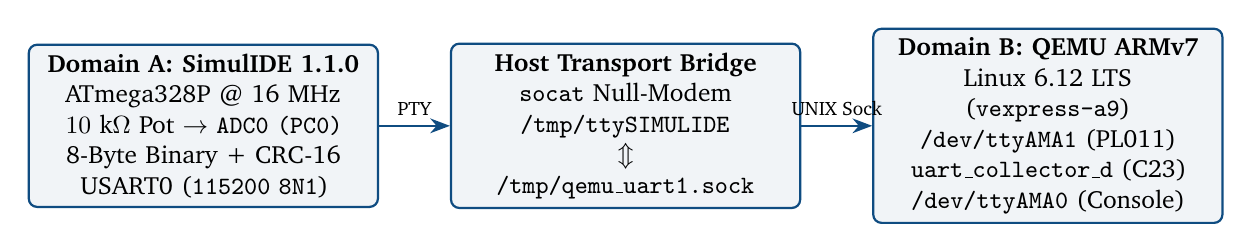
\begin{tikzpicture}[
    node distance=0.85cm and 0.9cm,
    box/.style={rectangle, draw=primary, thick, fill=primary!6, rounded corners=3pt, text width=4.2cm, align=center, minimum height=1.5cm, font=\small},
    arrow/.style={-{Stealth[length=2.5mm]}, thick, draw=primary}
]
\node[box] (sim) {\textbf{Domain A: SimulIDE 1.1.0}\\ATmega328P @ 16 MHz\\$10\text{ k}\Omega$ Pot $\rightarrow$ \texttt{ADC0 (PC0)}\\8-Byte Binary + CRC-16\\USART0 (\texttt{115200 8N1})};
\node[box, right=of sim] (bridge) {\textbf{Host Transport Bridge}\\\texttt{socat} Null-Modem\\\texttt{/tmp/ttySIMULIDE}\\$\Updownarrow$\\\texttt{/tmp/qemu\_uart1.sock}};
\node[box, right=of bridge] (qemu) {\textbf{Domain B: QEMU ARMv7}\\Linux 6.12 LTS (\texttt{vexpress-a9})\\\texttt{/dev/ttyAMA1} (PL011)\\\texttt{uart\_collector\_d} (C23)\\\texttt{/dev/ttyAMA0} (Console)};

\draw[arrow] (sim) -- node[above, font=\scriptsize] {PTY} (bridge);
\draw[arrow] (bridge) -- node[above, font=\scriptsize] {UNIX Sock} (qemu);
\end{tikzpicture}
\caption{End-to-end Hardware-in-the-Loop (HIL) co-simulation topology bridging SimulIDE 1.1.0 and QEMU ARMv7.}
\label{fig:ch1_hil_topology}
\end{figure}

\section{System-Level Requirements and Quality Attributes}

To satisfy production embedded engineering rigor, the implementation enforces six non-negotiable invariants across both domains:

\begin{table}[!htbp]
\centering
\caption{System-level engineering invariants enforced across Project 03.}
\label{tab:ch1_invariants}
\begin{tabularx}{\linewidth}{l l X}
\toprule
\textbf{Attribute} & \textbf{Domain} & \textbf{Enforced Engineering Mechanism} \\
\midrule
Zero Arduino HAL & AVR Firmware & Direct register manipulation via \texttt{<avr/io.h>} (\texttt{ADMUX}, \texttt{ADCSRA}, \texttt{UCSR0A/B/C}, \texttt{UBRR0H/L}, \texttt{DDRB}, \texttt{PORTB}); zero Arduino C++ runtime overhead. \\
Wire Integrity & Protocol & Fixed 8-byte Little-Endian binary frame with \texttt{0xAA 0x55} sync header and \texttt{CRC-16/CCITT-FALSE} over bytes \texttt{0..5}. \\
Zero-Heap Runtime & Linux Daemon & 512-byte static power-of-two \texttt{ring\_buffer\_t} allocated on the stack; zero \texttt{malloc()}/\texttt{free()} calls in the continuous event loop (MISRA C:2025) \cite{misra2025}. \\
Overflow Safety & Linux Daemon & ISO C23 \texttt{<stdckdint.h>} checked arithmetic (\texttt{ckd\_add}, \texttt{ckd\_mul}) and \texttt{[[nodiscard]]} return contracts \cite{gustedt2025,cppref_numeric}. \\
Event-Driven I/O & Linux Daemon & Non-blocking raw \texttt{termios} coupled with Linux \texttt{epoll\_wait()} ($0\%$ idle CPU, $O(1)$ interrupt wakeup) \cite{man_termios,man_epoll}. \\
Rootless Packaging & Build Pipeline & \texttt{cpio --owner=+0:+0}, \texttt{sfdisk}, and \texttt{mtools} (\texttt{mcopy}) construct MBR FAT32 \texttt{sdcard.img} and \texttt{uInitramfs} with zero \texttt{sudo} privileges. \\
\bottomrule
\end{tabularx}
\end{table}

\section{Repository Organization and Architectural Separation}

Professional embedded repositories separate public header interfaces (\texttt{include/}), private translation units (\texttt{src/}), unit tests (\texttt{tests/}), hardware schematics (\texttt{circuit/}), build automation (\texttt{scripts/}), and formal documentation (\texttt{docs/}). Table~\ref{tab:ch1_repo} maps every directory and file in \texttt{p03-simulide-uart-posix-daemon}.

\begin{table}[!htbp]
\centering
\caption{Complete directory and file inventory of the Project 03 repository.}
\label{tab:ch1_repo}
\begin{tabularx}{\linewidth}{l X}
\toprule
\textbf{Path} & \textbf{Architectural Responsibility} \\
\midrule
\texttt{Makefile} & Top-level orchestrator exposing \texttt{demo}, \texttt{direct}, \texttt{bridge}, \texttt{test-inject}, \texttt{build}, \texttt{clean}, and \texttt{distclean}. \\
\texttt{.gitignore} & Excludes upstream trees (\texttt{sources/}, \texttt{Bootloader/}, \texttt{kernel/}, \texttt{rootfs/}, \texttt{images/}), \texttt{**/build/}, \texttt{*.hex}, \texttt{*.elf}, and \texttt{*.img}. \\
\texttt{circuit/sensor\_node.sim1} & Pre-wired SimulIDE 1.1.0 schematic (ATmega328P, $10\text{ k}\Omega$ pot, $220\,\Omega$ LED, \texttt{Serial Port} at \texttt{115200 8N1}). \\
\texttt{firmware\_avr/include/} & Public AVR headers: \texttt{frame.h}, \texttt{crc16.h}, \texttt{uart.h}, \texttt{adc.h}. \\
\texttt{firmware\_avr/src/} & Bare-metal C implementations: \texttt{main.c}, \texttt{uart.c}, \texttt{adc.c}, \texttt{crc16.c}. \\
\texttt{firmware\_avr/tests/} & Host Golden Test Vector verification (\texttt{test\_crc16.c}). \\
\texttt{user/uart\_collector/include/} & C23/POSIX headers: \texttt{c23\_compat.h}, \texttt{ring\_buffer.h}, \texttt{frame\_parser.h}, \texttt{serial\_port.h}. \\
\texttt{user/uart\_collector/src/} & Linux daemon implementation: \texttt{main.c}, \texttt{ring\_buffer.c}, \texttt{frame\_parser.c}, \texttt{serial\_port.c}. \\
\texttt{user/uart\_collector/tests/} & ASan/UBSan unit test suites: \texttt{test\_ring\_buffer.c}, \texttt{test\_parser.c}. \\
\texttt{scripts/01..07*.sh} & Idempotent Embedded Linux build, packaging, and QEMU Dual-UART launch scripts. \\
\bottomrule
\end{tabularx}
\end{table}

\section{Dual-UART Peripheral Map and DRAM Boot Layout on QEMU \texttt{vexpress-a9}}

The emulated \texttt{vexpress-a9} motherboard instantiates four ARM PrimeCell \textbf{PL011} UART controllers mapped into physical peripheral space \cite{qemu_vexpress}. During Linux kernel initialization, the \texttt{amba-pl011} driver binds all four MMIO blocks to \texttt{/dev/ttyAMA0} through \texttt{/dev/ttyAMA3} as detailed in Table~\ref{tab:ch1_pl011}.

\begin{table}[!htbp]
\centering
\caption{ARM PL011 UART MMIO addresses, GIC interrupts, and QEMU bindings on \texttt{vexpress-a9}.}
\label{tab:ch1_pl011}
\begin{tabularx}{\linewidth}{l l l l X}
\toprule
\textbf{Device Node} & \textbf{MMIO Base} & \textbf{IRQ} & \textbf{QEMU Argument} & \textbf{Functional Assignment} \\
\midrule
\texttt{/dev/ttyAMA0} & \texttt{0x10009000} & 38 & \texttt{-serial mon:stdio} & Kernel boot log and interactive BusyBox shell. \\
\texttt{/dev/ttyAMA1} & \texttt{0x1000a000} & 39 & \texttt{-serial chardev:uart1} & Binary sensor telemetry input bridged from \texttt{/tmp/qemu\_uart1.sock}. \\
\texttt{/dev/ttyAMA2} & \texttt{0x1000b000} & 40 & *(Unconnected)* & Exposed by DTB, unused in Project 03. \\
\texttt{/dev/ttyAMA3} & \texttt{0x1000c000} & 41 & *(Unconnected)* & Exposed by DTB, unused in Project 03. \\
\bottomrule
\end{tabularx}
\end{table}

DDR2 physical memory (\emph{DRAM Bank 0}) starts at \texttt{0x60000000} and spans $512\text{ MiB}$ (\texttt{0x60000000}--\texttt{0x7FFFFFFF}). U-Boot stages \texttt{boot.scr} at \texttt{0x60000000}, loads \texttt{zImage} at \texttt{0x60100000}, \texttt{vexpress-v2p-ca9.dtb} at \texttt{0x62000000}, and \texttt{uInitramfs} at \texttt{0x63000000}, preventing any payload overlap during kernel decompression.


\chapter{Binary Wire Protocol, Struct Packing, Endianness, and CRC-16/CCITT-FALSE}

\section{Binary Framing Versus ASCII Text Protocols}

When designing an embedded serial protocol between an 8-bit microcontroller and a Linux host, engineers choose between human-readable ASCII lines (e.g., \texttt{"SEQ:1,ADC:512\textbackslash n"}) and fixed-length binary frames. Table~\ref{tab:ch2_bin_vs_ascii} summarizes why Project 03 mandates a fixed 8-byte binary frame.

\begin{table}[!htbp]
\centering
\caption{Engineering comparison: fixed 8-byte binary frame vs. ASCII text telemetry.}
\label{tab:ch2_bin_vs_ascii}
\begin{tabularx}{\linewidth}{l X X}
\toprule
\textbf{Metric} & \textbf{ASCII Text Line} & \textbf{8-Byte Binary Frame (Project 03)} \\
\midrule
Wire Payload Size & Variable ($16\text{--}28$ bytes per sample) & Fixed \textbf{8 bytes} ($694\,\mu\text{s}$ at \texttt{115200 8N1}) \\
MCU Flash Cost & High ($>1.5\text{ KiB}$ for \texttt{snprintf}) & Minimal ($<100$ bytes for struct copy) \\
Error Detection & None unless manual ASCII hex CRC appended & Hardware-grade \textbf{CRC-16/CCITT-FALSE} \\
Parser Complexity & String tokenization (\texttt{strtok}/\texttt{sscanf}) & Constant-time FSM + \texttt{read\_u16\_le()} \\
Resynchronization & Relies on \texttt{\textbackslash n} (corrupted newline merges packets) & Dual sync bytes (\texttt{0xAA 0x55}) + CRC verification \\
\bottomrule
\end{tabularx}
\end{table}

\section{Endianness (Byte Ordering) and Cross-Architecture Portability}

A UART peripheral transmits exactly \textbf{one byte (8 bits)} per frame. Consequently, any 16-bit integer such as \texttt{adc\_raw = 512} (\texttt{0x0200}) must be split into two consecutive bytes on the wire:
\begin{itemize}
\item \textbf{Little-Endian (Least Significant Byte first):} Byte 0 is \texttt{0x00} (low byte) and Byte 1 is \texttt{0x02} (high byte). Both the AVR ATmega328P and ARMv7 Cortex-A9 in Linux use Little-Endian representation natively.
\item \textbf{Big-Endian (Most Significant Byte first):} Byte 0 is \texttt{0x02} and Byte 1 is \texttt{0x00} (used by TCP/IP headers).
\end{itemize}

If a transmitter sends Big-Endian while the receiver interprets Little-Endian without explicit conversion, \texttt{0x0200} ($512$) is silently misread as \texttt{0x0002} ($2$). Project 03 locks the wire specification strictly to \textbf{Little-Endian} and decodes every 16-bit field explicitly on the Linux receiver using bit shifts:
\[
\text{value}_{16} = \text{buf}[0] \;\big|\; \bigl(\text{buf}[1] \ll 8\bigr)
\]
This makes the Linux parser completely independent of the host CPU's native endianness.

\section{Deep Dive into \texttt{typedef struct \_\_attribute\_\_((packed))} and \texttt{\_Static\_assert}}

Listing~\ref{lst:ch2_frame_h} presents the complete source code of \texttt{firmware\_avr/include/frame.h}.

\begin{lstlisting}[language=C,label=lst:ch2_frame_h,caption={Complete listing of \texttt{firmware\_avr/include/frame.h}.}]
/**
 * @file frame.h
 * @brief 8-byte binary UART telemetry frame definition (Little-Endian).
 *        Shared wire contract between the ATmega328P firmware and Linux daemon.
 */
#ifndef P02_FRAME_H
#define P02_FRAME_H

#include <stdint.h>

enum {
    FRAME_SOF_0      = 0xAAU,
    FRAME_SOF_1      = 0x55U,
    FRAME_SIZE_BYTES = 8U,
    FRAME_CRC_OFFSET = 6U
};

typedef struct __attribute__((packed)) {
    uint8_t  sof[2];    /* Start-of-Frame marker: 0xAA, 0x55 */
    uint16_t seq_id;    /* Little-Endian: monotonic packet sequence counter */
    uint16_t adc_raw;   /* Little-Endian: 10-bit ADC sample (0..1023) */
    uint16_t crc16;     /* Little-Endian: CRC-16/CCITT-FALSE over bytes 0..5 */
} telemetry_frame_t;

_Static_assert(sizeof(telemetry_frame_t) == FRAME_SIZE_BYTES,
               "telemetry_frame_t must be exactly 8 bytes");

#endif /* P02_FRAME_H */
\end{lstlisting}

\subsection{Why Natural Alignment and Structure Padding Break Wire Protocols}
In standard C, every scalar type has an alignment requirement \texttt{\_Alignof(T)} (typically equal to its size: 1 byte for \texttt{uint8\_t}, 2 bytes for \texttt{uint16\_t}, 4 bytes for \texttt{uint32\_t}). When laying out a \texttt{struct}, the compiler inserts unnamed \textbf{padding bytes} between fields and at the end of the structure so that each field starts at an address divisible by its alignment \cite{gustedt2025,seacord2020}. While padding improves memory bus throughput on 32-bit/64-bit CPUs, it introduces two severe hazards in wire protocols:
\begin{enumerate}
\item \textbf{Layout Drift Across Architectures:} The same unpacked C struct can have different byte sizes on an 8-bit AVR versus a 32-bit ARM or 64-bit x86\_64 CPU.
\item \textbf{Uninitialized Information Leakage:} Padding bytes are not guaranteed to be zero-initialized, causing random stack contents to be transmitted over UART and invalidating CRC calculations.
\end{enumerate}

\subsection{How \texttt{\_\_attribute\_\_((packed))} Works and Its Alignment Trade-Off}
Attaching \texttt{\_\_attribute\_\_((packed))} to the \texttt{struct} instructs GCC/Clang to override natural alignment and pack every member at 1-byte boundaries with zero internal or trailing padding.
\begin{itemize}
\item \textbf{On ATmega328P (8-bit AVR):} The data bus is 8 bits wide; every memory access is inherently 1-byte aligned, so \texttt{packed} incurs \textbf{zero runtime overhead}.
\item \textbf{On ARMv7 Cortex-A9 (32-bit Linux):} Casting an arbitrary unaligned \texttt{uint8\_t *} pointer inside a ring buffer to \texttt{telemetry\_frame\_t *} risks unaligned access penalties or undefined behavior under strict aliasing (\texttt{-fstrict-aliasing}) \cite{seacord2020}. For this reason, our Linux daemon \emph{never} casts raw buffer memory to a packed struct; it copies 8 bytes into a local array and reconstructs each 16-bit integer explicitly via \texttt{read\_u16\_le()}.
\end{itemize}

\subsection{Compile-Time Contract Enforcement via \texttt{\_Static\_assert}}
The declaration \texttt{\_Static\_assert(sizeof(telemetry\_frame\_t) == FRAME\_SIZE\_BYTES, ...)} is evaluated by the compiler front-end before code generation \cite{gustedt2025}. It produces zero runtime code and acts as a permanent mathematical guard: if any developer modifies a field type (e.g., changing \texttt{seq\_id} to \texttt{uint32\_t}) without updating the protocol specification, compilation immediately aborts with an explicit error message.

\section{Mathematical Derivation of CRC-16/CCITT-FALSE over $GF(2)$}

\subsection{Polynomial Arithmetic in the Galois Field $GF(2)$}
A Cyclic Redundancy Check interprets an $n$-bit message $b_{n-1} b_{n-2} \dots b_1 b_0$ as a polynomial with binary coefficients in the finite field $GF(2) = (\{0, 1\}, +, \cdot)$:
\[
M(x) = \sum_{i=0}^{n-1} b_i x^i \in GF(2)[x]
\]
In $GF(2)$, arithmetic is performed modulo 2 with \textbf{no carries and no borrows}:
\[
0 + 0 = 0, \quad 0 + 1 = 1, \quad 1 + 0 = 1, \quad 1 + 1 = 0
\]
Consequently, both polynomial addition and polynomial subtraction are identically the CPU \textbf{bitwise XOR ($\oplus$)} instruction. Multiplying a polynomial by $x$ corresponds to a \textbf{left bit shift by 1 (\texttt{<< 1})}.

\subsection{Generator Polynomial \texttt{0x1021} and CCITT-FALSE Parameters}
The \textbf{CRC-16/CCITT-FALSE} standard (widely deployed in X.25, HDLC, Bluetooth, and industrial telemetry) is defined by five exact parameters:

\begin{table}[!htbp]
\centering
\caption{Formal parameter specification of CRC-16/CCITT-FALSE.}
\label{tab:ch2_crc_params}
\begin{tabularx}{\linewidth}{l l X}
\toprule
\textbf{Parameter} & \textbf{Value} & \textbf{Mathematical \& Engineering Role Engineering Role} \\
\midrule
Width & 16 bits & Produces a 16-bit remainder ($65\,536$ possible states). \\
Polynomial $G(x)$ & \texttt{0x1021} & Represents $x^{16} + x^{12} + x^5 + 1$ (implicit $x^{16}$ omitted in 16-bit representation). \\
Initial Value (\texttt{Init}) & \texttt{0xFFFF} & Non-zero seed ensures leading \texttt{0x00} bytes alter the final remainder. \\
\texttt{RefIn} / \texttt{RefOut} & \texttt{false} / \texttt{false} & Processes each byte MSB-first without bit-reversal. \\
Final XOR (\texttt{XorOut}) & \texttt{0x0000} & Remainder is output directly without final inversion. \\
\bottomrule
\end{tabularx}
\end{table}

When the transmitter appends the 16-bit remainder $R(x) = \bigl(M(x)\cdot x^{16}\bigr) \bmod G(x)$, any transmission error adds an error polynomial $E(x)$ on the wire, yielding $T'(x) = T(x) \oplus E(x)$. The receiver detects the error whenever $E(x)$ is not evenly divisible by $G(x)$. Because $G(x) = x^{16} + x^{12} + x^5 + 1 = (x+1)(x^{15}+x^{14}+x^{13}+x^{12}+x^4+x^3+x^2+x+1)$:
\begin{itemize}
\item Any single-bit error $E(x) = x^k$ is never divisible by $G(x)$ (100\% detected).
\item Any odd number of bit errors has $E(1) = 1 \neq 0$, so $(x+1) \nmid E(x)$ (100\% detected).
\item Any burst error of length $L \le 16$ has form $E(x) = x^k B(x)$ with $\deg(B) < 16 = \deg(G)$, so $G(x) \nmid E(x)$ (100\% detected).
\end{itemize}

\subsection{Complete Bit-by-Bit Trace of the Golden Test Vector}

Table~\ref{tab:ch2_crc_trace} records all 48 shift-and-XOR steps executed by \texttt{crc16\_ccitt\_false()} on our 6-byte Golden Test Vector \texttt{AA 55 01 00 00 02} (\texttt{seq\_id = 1}, \texttt{adc\_raw = 512}), mathematically confirming the final value \textbf{\texttt{0x09A9}} (transmitted Little-Endian as \texttt{A9 09}).

\begin{longtable}{l c c c c l c}
\caption{Complete 48-step bit-by-bit trace of CRC-16/CCITT-FALSE on \texttt{AA 55 01 00 00 02}.}
\label{tab:ch2_crc_trace} \\
\toprule
\textbf{Input Byte} & \textbf{CRC In} & \textbf{After XOR} & \textbf{Bit} & \textbf{MSB} & \textbf{Operation} & \textbf{CRC Out} \\
\midrule
\endfirsthead
\toprule
\textbf{Input Byte} & \textbf{CRC In} & \textbf{After XOR} & \textbf{Bit} & \textbf{MSB} & \textbf{Operation} & \textbf{CRC Out} \\
\midrule
\endhead
\bottomrule
\endfoot
Byte 0 (\texttt{0xAA}) & \texttt{0xFFFF} & \texttt{0x55FF} & 0 & 0 & \texttt{<<1} & \texttt{0xABFE} \\
 &  &  & 1 & 1 & \texttt{<<1 \^{} 0x1021} & \texttt{0x47DD} \\
 &  &  & 2 & 0 & \texttt{<<1} & \texttt{0x8FBA} \\
 &  &  & 3 & 1 & \texttt{<<1 \^{} 0x1021} & \texttt{0x0F55} \\
 &  &  & 4 & 0 & \texttt{<<1} & \texttt{0x1EAA} \\
 &  &  & 5 & 0 & \texttt{<<1} & \texttt{0x3D54} \\
 &  &  & 6 & 0 & \texttt{<<1} & \texttt{0x7AA8} \\
 &  &  & 7 & 0 & \texttt{<<1} & \texttt{0xF550} \\
\midrule
Byte 1 (\texttt{0x55}) & \texttt{0xF550} & \texttt{0xA050} & 0 & 1 & \texttt{<<1 \^{} 0x1021} & \texttt{0x5081} \\
 &  &  & 1 & 0 & \texttt{<<1} & \texttt{0xA102} \\
 &  &  & 2 & 1 & \texttt{<<1 \^{} 0x1021} & \texttt{0x5225} \\
 &  &  & 3 & 0 & \texttt{<<1} & \texttt{0xA44A} \\
 &  &  & 4 & 1 & \texttt{<<1 \^{} 0x1021} & \texttt{0x58B5} \\
 &  &  & 5 & 0 & \texttt{<<1} & \texttt{0xB16A} \\
 &  &  & 6 & 1 & \texttt{<<1 \^{} 0x1021} & \texttt{0x72F5} \\
 &  &  & 7 & 0 & \texttt{<<1} & \texttt{0xE5EA} \\
\midrule
Byte 2 (\texttt{0x01}) & \texttt{0xE5EA} & \texttt{0xE4EA} & 0 & 1 & \texttt{<<1 \^{} 0x1021} & \texttt{0xD9F5} \\
 &  &  & 1 & 1 & \texttt{<<1 \^{} 0x1021} & \texttt{0xA3CB} \\
 &  &  & 2 & 1 & \texttt{<<1 \^{} 0x1021} & \texttt{0x57B7} \\
 &  &  & 3 & 0 & \texttt{<<1} & \texttt{0xAF6E} \\
 &  &  & 4 & 1 & \texttt{<<1 \^{} 0x1021} & \texttt{0x4EFD} \\
 &  &  & 5 & 0 & \texttt{<<1} & \texttt{0x9DFA} \\
 &  &  & 6 & 1 & \texttt{<<1 \^{} 0x1021} & \texttt{0x2BD5} \\
 &  &  & 7 & 0 & \texttt{<<1} & \texttt{0x57AA} \\
\midrule
Byte 3 (\texttt{0x00}) & \texttt{0x57AA} & \texttt{0x57AA} & 0 & 0 & \texttt{<<1} & \texttt{0xAF54} \\
 &  &  & 1 & 1 & \texttt{<<1 \^{} 0x1021} & \texttt{0x4E89} \\
 &  &  & 2 & 0 & \texttt{<<1} & \texttt{0x9D12} \\
 &  &  & 3 & 1 & \texttt{<<1 \^{} 0x1021} & \texttt{0x2A05} \\
 &  &  & 4 & 0 & \texttt{<<1} & \texttt{0x540A} \\
 &  &  & 5 & 0 & \texttt{<<1} & \texttt{0xA814} \\
 &  &  & 6 & 1 & \texttt{<<1 \^{} 0x1021} & \texttt{0x4009} \\
 &  &  & 7 & 0 & \texttt{<<1} & \texttt{0x8012} \\
\midrule
Byte 4 (\texttt{0x00}) & \texttt{0x8012} & \texttt{0x8012} & 0 & 1 & \texttt{<<1 \^{} 0x1021} & \texttt{0x1005} \\
 &  &  & 1 & 0 & \texttt{<<1} & \texttt{0x200A} \\
 &  &  & 2 & 0 & \texttt{<<1} & \texttt{0x4014} \\
 &  &  & 3 & 0 & \texttt{<<1} & \texttt{0x8028} \\
 &  &  & 4 & 1 & \texttt{<<1 \^{} 0x1021} & \texttt{0x1071} \\
 &  &  & 5 & 0 & \texttt{<<1} & \texttt{0x20E2} \\
 &  &  & 6 & 0 & \texttt{<<1} & \texttt{0x41C4} \\
 &  &  & 7 & 0 & \texttt{<<1} & \texttt{0x8388} \\
\midrule
Byte 5 (\texttt{0x02}) & \texttt{0x8388} & \texttt{0x8188} & 0 & 1 & \texttt{<<1 \^{} 0x1021} & \texttt{0x1331} \\
 &  &  & 1 & 0 & \texttt{<<1} & \texttt{0x2662} \\
 &  &  & 2 & 0 & \texttt{<<1} & \texttt{0x4CC4} \\
 &  &  & 3 & 0 & \texttt{<<1} & \texttt{0x9988} \\
 &  &  & 4 & 1 & \texttt{<<1 \^{} 0x1021} & \texttt{0x2331} \\
 &  &  & 5 & 0 & \texttt{<<1} & \texttt{0x4662} \\
 &  &  & 6 & 0 & \texttt{<<1} & \texttt{0x8CC4} \\
 &  &  & 7 & 1 & \texttt{<<1 \^{} 0x1021} & \texttt{0x09A9} \\
\end{longtable}


\chapter{Internals of \texttt{<avr/io.h>} and Complete ATmega328P Register Reference}

\section{How \texttt{<avr/io.h>} Works Under the Hood}

To a developer accustomed to desktop C programming, statements such as \texttt{ADMUX = (uint8\_t)(1U << REFS0);} or \texttt{UCSR0B = (uint8\_t)((1U << TXEN0) | (1U << RXEN0));} can appear mysterious because \texttt{ADMUX} and \texttt{UCSR0B} are never declared as local or global variables in the user's source files. Understanding how \texttt{avr-libc} implements \texttt{<avr/io.h>} demystifies all bare-metal microcontroller programming \cite{avr_libc_io,avr_libc_sfr}.

\subsection{Step 1: Compiler Target Selection (\texttt{-mmcu=atmega328p})}
When \texttt{avr-gcc} compiles with \texttt{-mmcu=atmega328p}, the compiler driver automatically injects the predefined macro \texttt{\_\_AVR\_ATmega328P\_\_} into the preprocessor symbol table. Inside \texttt{/usr/lib/avr/include/avr/io.h}, a large dispatch chain checks these macros:

\begin{lstlisting}[language=C,caption={Simplified internal dispatch mechanism inside \texttt{<avr/io.h>} (\texttt{avr-libc}).}]
#include <avr/sfr_defs.h>

#if defined (__AVR_ATmega328P__)
#  include <avr/iom328p.h>
#elif defined (__AVR_ATmega2560__)
#  include <avr/iom2560.h>
/* ... hundreds of other AVR silicon variants ... */
#else
#  warning "device type not defined"
#endif
\end{lstlisting}

\subsection{Step 2: Memory-Mapped I/O (MMIO) and Special Function Registers (SFRs)}
The ATmega328P uses a modified Harvard architecture with an 8-bit data address space \cite{microchip_328p}:
\begin{itemize}
\item \texttt{0x0000}--\texttt{0x001F}: 32 General Purpose Working Registers (\texttt{R0}--\texttt{R31}).
\item \texttt{0x0020}--\texttt{0x005F}: 64 Standard I/O Registers (accessible via single-cycle \texttt{IN}/\texttt{OUT} instructions, offset by \texttt{0x20} from their I/O address). Includes \texttt{DDRB} (\texttt{0x04} I/O / \texttt{0x24} memory) and \texttt{PORTB} (\texttt{0x05} I/O / \texttt{0x25} memory).
\item \texttt{0x0060}--\texttt{0x00FF}: 160 Extended I/O Registers (accessible via \texttt{LDS}/\texttt{STS} memory instructions). Includes all ADC registers (\texttt{0x78}--\texttt{0x7C}) and all USART0 registers (\texttt{0xC0}--\texttt{0xC6}).
\item \texttt{0x0100}--\texttt{0x08FF}: $2048$ bytes ($2\text{ KiB}$) of internal SRAM.
\end{itemize}

Inside \texttt{<avr/sfr\_defs.h>} \cite{avr_libc_sfr}, the macros \texttt{\_SFR\_IO8} and \texttt{\_SFR\_MEM8} translate raw integer silicon addresses into dereferenced \texttt{volatile} C pointers:

\begin{lstlisting}[language=C,caption={Exact pointer-dereference expansion of SFR macros in \texttt{<avr/sfr\_defs.h>}.}]
#define _MMIO_BYTE(mem_addr) (*(volatile uint8_t *)(mem_addr))
#define _MMIO_WORD(mem_addr) (*(volatile uint16_t *)(mem_addr))

#define _SFR_IO8(io_addr)    _MMIO_BYTE((io_addr) + 0x20)
#define _SFR_MEM8(mem_addr)  _MMIO_BYTE(mem_addr)
#define _SFR_MEM16(mem_addr) _MMIO_WORD(mem_addr)
\end{lstlisting}

Therefore, when \texttt{<avr/iom328p.h>} writes \texttt{\#define ADMUX \_SFR\_MEM8(0x7C)} and \texttt{\#define REFS0 6}, the C statement:
\begin{lstlisting}[language=C]
ADMUX = (uint8_t)(1U << REFS0);
\end{lstlisting}
is preprocessed directly into:
\begin{lstlisting}[language=C]
(*(volatile uint8_t *)(0x7C)) = (uint8_t)(1U << 6); /* Writes 0x40 to address 0x7C */
\end{lstlisting}

\subsection{Step 3: Why \texttt{volatile} Is Mandatory on Hardware Registers}
The C \texttt{volatile} type qualifier tells the compiler optimizer that the value stored at that memory address may change at any time due to external silicon activity (an ADC conversion finishing, a UART shift register emptying, or a GPIO pin changing voltage) without any visible C code writing to it \cite{gustedt2025,seacord2020}.
\begin{itemize}
\item Without \texttt{volatile}, \texttt{avr-gcc -Os} would optimize \texttt{while ((ADCSRA \& (1U << ADSC)) != 0U) \{\}} into reading \texttt{ADCSRA} once into register \texttt{R24} and looping forever on \texttt{R24}, hanging the MCU.
\item With \texttt{volatile}, the compiler emits an \texttt{LDS} instruction inside the loop body on every iteration so the CPU continuously polls the live silicon flip-flop.
\end{itemize}

\subsection{Step 4: Bitwise Idioms Used in Bare-Metal C}
Every register manipulation in \texttt{adc.c}, \texttt{uart.c}, and \texttt{main.c} relies on four standard C bitwise patterns:
\begin{enumerate}
\item \textbf{Set a bit (1) without modifying others:} \texttt{REG |= (uint8\_t)(1U << BIT);} (e.g., \texttt{ADCSRA |= (uint8\_t)(1U << ADSC);}).
\item \textbf{Clear a bit (0) without modifying others:} \texttt{REG \&= (uint8\_t)\textasciitilde(1U << BIT);} (e.g., turning off LED on \texttt{PORTB5}).
\item \textbf{Test whether a bit is 1:} \texttt{(REG \& (uint8\_t)(1U << BIT)) != 0U} (e.g., polling \texttt{ADSC} or \texttt{UDRE0}).
\item \textbf{Replace a multi-bit field safely (Read-Modify-Write):} \texttt{REG = (uint8\_t)((REG \& MASK\_KEEP) | (VAL \& MASK\_NEW));} (e.g., updating channel bits \texttt{MUX3:0} inside \texttt{ADMUX} while preserving \texttt{REFS1:0}).
\end{enumerate}

\section{Complete Register-by-Register Specification: GPIO Port B}

In \texttt{firmware\_avr/src/main.c}, the TX activity LED is wired to Arduino Pin 13, which corresponds to physical pin \textbf{PB5} (Port B, bit 5) of the ATmega328P \cite{microchip_328p}.

\begin{table}[!htbp]
\centering
\caption{ATmega328P Port B GPIO registers used to drive the TX activity LED.}
\label{tab:ch3_gpio}
\begin{tabularx}{\linewidth}{l l l X}
\toprule
\textbf{Register / Bit} & \textbf{Address} & \textbf{Reset} & \textbf{Detailed Hardware Behavior} \\
\midrule
\texttt{DDRB} & \texttt{0x24} (\texttt{0x04} I/O) & \texttt{0x00} & \textbf{Port B Data Direction Register}: Each bit $n \in [0..7]$ sets pin \texttt{PBn} as Input (\texttt{0}) or Output (\texttt{1}). \\
\texttt{DDB5} & Bit 5 of \texttt{DDRB} & \texttt{0} & Setting \texttt{DDRB |= (1U << DDB5)} configures \texttt{PB5} (Pin 13) as a push-pull $5\text{ V}$ CMOS output driver. \\
\texttt{PORTB} & \texttt{0x25} (\texttt{0x05} I/O) & \texttt{0x00} & \textbf{Port B Data Register}: When \texttt{DDBn = 1}, writing \texttt{1} drives \texttt{PBn} to $V_{\text{CC}}$ ($5\text{ V}$); writing \texttt{0} drives it to \texttt{GND} ($0\text{ V}$). \\
\texttt{PORTB5} & Bit 5 of \texttt{PORTB} & \texttt{0} & Driven HIGH at the start of every telemetry sample to light the LED for $40\text{ ms}$, then cleared LOW. \\
\bottomrule
\end{tabularx}
\end{table}

\section{Complete Register-by-Register Specification: 10-Bit ADC Peripheral}

The ATmega328P integrates a 10-bit successive-approximation Analog-to-Digital Converter (ADC) producing integer readings from \texttt{0} ($0\text{ V}$) to \texttt{1023} ($V_{\text{REF}} - 1\text{ LSB}$) \cite{microchip_328p}. Every register and every single bit inside \texttt{ADMUX}, \texttt{ADCSRA}, and \texttt{ADC} is broken down below.

\subsection{\texttt{ADMUX} --- ADC Multiplexer Selection Register (Address \texttt{0x7C})}

\begin{table}[!htbp]
\centering
\caption{Complete 8-bit layout of \texttt{ADMUX} (\texttt{0x7C}) and exact values configured in \texttt{adc.c}.}
\label{tab:ch3_admux}
\begin{tabularx}{\linewidth}{c l c X}
\toprule
\textbf{Bit} & \textbf{Symbol} & \textbf{Project 03 Value} & \textbf{Complete Hardware Specification} \\
\midrule
7 & \texttt{REFS1} & \texttt{0} & \textbf{Reference Selection Bit 1}: Together with \texttt{REFS0}, selects the ADC full-scale voltage reference: \texttt{00} = external \texttt{AREF}; \texttt{01} = \texttt{AVCC} ($5\text{ V}$ with cap on \texttt{AREF}); \texttt{10} = reserved; \texttt{11} = internal $1.1\text{ V}$ bandgap. \\
6 & \texttt{REFS0} & \texttt{1} & \textbf{Reference Selection Bit 0}: Setting \texttt{REFS1:0 = 01b} via \texttt{ADMUX = (1U << REFS0)} ties full-scale \texttt{1023} to the $5\text{ V}$ \texttt{AVCC} rail powering our $10\text{ k}\Omega$ potentiometer. \\
5 & \texttt{ADLAR} & \texttt{0} & \textbf{ADC Left Adjust Result}: \texttt{0} right-adjusts the 10-bit result into \texttt{ADCH[1:0]:ADCL[7:0]} so reading \texttt{ADC} directly yields \texttt{0..1023}. \\
4 & *(Res)* & \texttt{0} & Reserved bit; always written \texttt{0}. \\
3..0 & \texttt{MUX3:0} & \texttt{0000b} & \textbf{Analog Channel Selection Bits}: Selects which analog pin connects to the sample-and-hold capacitor (\texttt{0000b} = \texttt{ADC0 / PC0}, \texttt{0001b} = \texttt{ADC1}, \dots, \texttt{0111b} = \texttt{ADC7}). Updated safely via \texttt{(ADMUX \& 0xF0U) | (channel \& 0x07U)}. \\
\bottomrule
\end{tabularx}
\end{table}

\subsection{\texttt{ADCSRA} --- ADC Control and Status Register A (Address \texttt{0x7A})}

\begin{table}[!htbp]
\centering
\caption{Complete 8-bit layout of \texttt{ADCSRA} (\texttt{0x7A}) and exact values configured in \texttt{adc.c}.}
\label{tab:ch3_adcsra}
\begin{tabularx}{\linewidth}{c l c X}
\toprule
\textbf{Bit} & \textbf{Symbol} & \textbf{Project 03 Value} & \textbf{Complete Hardware Specification} \\
\midrule
7 & \texttt{ADEN} & \texttt{1} & \textbf{ADC Enable}: Writing \texttt{1} powers on the analog ADC core and internal comparator. Writing \texttt{0} disables it to reduce sleep current. \\
6 & \texttt{ADSC} & \texttt{1} (trigger) & \textbf{ADC Start Conversion}: In single-conversion mode, writing \texttt{1} starts one conversion (25 ADC clocks on the very first conversion, 13 ADC clocks thereafter). Hardware holds \texttt{ADSC = 1} while busy and clears it to \texttt{0} automatically when finished. \\
5 & \texttt{ADATE} & \texttt{0} & \textbf{ADC Auto Trigger Enable}: \texttt{0} disables free-running/timer triggers so conversions happen strictly on demand inside \texttt{adc\_read\_channel()}. \\
4 & \texttt{ADIF} & \texttt{0} & \textbf{ADC Interrupt Flag}: Set by hardware when a conversion completes. Not needed when polling \texttt{ADSC}. \\
3 & \texttt{ADIE} & \texttt{0} & \textbf{ADC Interrupt Enable}: \texttt{0} keeps ADC interrupts disabled (we use deterministic polling). \\
2 & \texttt{ADPS2} & \texttt{1} & \textbf{ADC Prescaler Bit 2}: Together with \texttt{ADPS1:0}, divides $F_{\text{CPU}}$ to generate the ADC successive-approximation clock. \\
1 & \texttt{ADPS1} & \texttt{1} & \textbf{ADC Prescaler Bit 1}: Part of the 3-bit division factor ($2, 2, 4, 8, 16, 32, 64, 128$). \\
0 & \texttt{ADPS0} & \texttt{1} & \textbf{ADC Prescaler Bit 0}: \texttt{ADPS2:0 = 111b} selects division by \textbf{128}, yielding $f_{\text{ADC}} = 16\text{ MHz} / 128 = 125\text{ kHz}$ (strictly inside the datasheet's $50\text{--}200\text{ kHz}$ precision band). \\
\bottomrule
\end{tabularx}
\end{table}

\subsection{\texttt{ADCL} (\texttt{0x78}), \texttt{ADCH} (\texttt{0x79}), and the 16-Bit \texttt{ADC} Macro}

Because the ATmega328P is an 8-bit CPU, a 10-bit ADC result spans two 8-bit registers: \texttt{ADCL} (bits 7..0) and \texttt{ADCH} (bits 9..8). According to the ATmega328P datasheet \cite{microchip_328p}, reading \texttt{ADCL} locks both registers so a new conversion cannot overwrite \texttt{ADCH} mid-read; reading \texttt{ADCH} unlocks them. If software read \texttt{ADCH} first, the lock would never engage or release properly. In \texttt{avr-libc}, the 16-bit macro \texttt{ADC} expands to \texttt{\_SFR\_MEM16(0x78)}, and \texttt{avr-gcc} guarantees that reading a 16-bit Little-Endian SFR always loads the low byte (\texttt{ADCL}, \texttt{0x78}) first and the high byte (\texttt{ADCH}, \texttt{0x79}) second.

\section{Complete Register-by-Register Specification: USART0 Peripheral}

The ATmega328P's hardware serial engine (\textbf{USART0}) drives pin \texttt{PD1 (TXD)} and samples pin \texttt{PD0 (RXD)} using five primary control/data registers \cite{microchip_328p}.

\subsection{\texttt{UCSR0A} --- USART Control and Status Register 0A (Address \texttt{0xC0})}

\begin{table}[!htbp]
\centering
\caption{Complete 8-bit layout of \texttt{UCSR0A} (\texttt{0xC0}).}
\label{tab:ch3_ucsr0a}
\begin{tabularx}{\linewidth}{c l c X}
\toprule
\textbf{Bit} & \textbf{Symbol} & \textbf{Project 03 Value} & \textbf{Complete Hardware Specification} \\
\midrule
7 & \texttt{RXC0} & Read-only & \textbf{USART Receive Complete}: \texttt{1} when unread data sits in the RX buffer. \\
6 & \texttt{TXC0} & \texttt{0} & \textbf{USART Transmit Complete}: \texttt{1} when the entire shift register has shifted out and \texttt{UDR0} is empty. \\
5 & \texttt{UDRE0} & Polled & \textbf{USART Data Register Empty}: \texttt{1} when \texttt{UDR0} is ready to accept a new byte. \texttt{uart\_send\_byte()} spins on \texttt{(UCSR0A \& (1U << UDRE0)) == 0U} before writing \texttt{UDR0}. \\
4 & \texttt{FE0} & Read-only & \textbf{Frame Error}: \texttt{1} if the next RX byte had a missing stop bit. \\
3 & \texttt{DOR0} & Read-only & \textbf{Data OverRun}: \texttt{1} if an incoming RX byte was lost due to buffer overflow. \\
2 & \texttt{UPE0} & Read-only & \textbf{USART Parity Error}: \texttt{1} if parity checking failed (unused in 8N1). \\
1 & \texttt{U2X0} & \texttt{1} & \textbf{Double USART Transmission Speed}: Halves the baud rate divisor from $16$ to $8$. Essential at $16\text{ MHz}$ for \texttt{115200 bps} (reduces clock error from $-3.55\%$ to $+2.12\%$). \\
0 & \texttt{MPCM0} & \texttt{0} & \textbf{Multi-Processor Communication Mode}: \texttt{0} disables multi-drop address filtering. \\
\bottomrule
\end{tabularx}
\end{table}

\subsection{\texttt{UCSR0B} --- USART Control and Status Register 0B (Address \texttt{0xC1})}

\begin{table}[!htbp]
\centering
\caption{Complete 8-bit layout of \texttt{UCSR0B} (\texttt{0xC1}).}
\label{tab:ch3_ucsr0b}
\begin{tabularx}{\linewidth}{c l c X}
\toprule
\textbf{Bit} & \textbf{Symbol} & \textbf{Project 03 Value} & \textbf{Complete Hardware Specification} \\
\midrule
7 & \texttt{RXCIE0} & \texttt{0} & \textbf{RX Complete Interrupt Enable}: \texttt{0} disables RX ISR. \\
6 & \texttt{TXCIE0} & \texttt{0} & \textbf{TX Complete Interrupt Enable}: \texttt{0} disables TX-done ISR. \\
5 & \texttt{UDRIE0} & \texttt{0} & \textbf{Data Register Empty Interrupt Enable}: \texttt{0} (we poll \texttt{UDRE0}). \\
4 & \texttt{RXEN0} & \texttt{1} & \textbf{Receiver Enable}: Overrides GPIO on pin \texttt{PD0} and enables the USART0 receiver logic. \\
3 & \texttt{TXEN0} & \texttt{1} & \textbf{Transmitter Enable}: Overrides GPIO on pin \texttt{PD1} and enables the USART0 transmitter shift register. \\
2 & \texttt{UCSZ02} & \texttt{0} & \textbf{Character Size Bit 2}: Combined with \texttt{UCSZ01:0 = 11b} in \texttt{UCSR0C} to select 8-bit frames (\texttt{011b}). \\
1 & \texttt{RXB80} & \texttt{0} & 9th received data bit (unused in 8-bit mode). \\
0 & \texttt{TXB80} & \texttt{0} & 9th transmitted data bit (unused in 8-bit mode). \\
\bottomrule
\end{tabularx}
\end{table}

\subsection{\texttt{UCSR0C} (\texttt{0xC2}), \texttt{UBRR0H} (\texttt{0xC5}), \texttt{UBRR0L} (\texttt{0xC4}), and \texttt{UDR0} (\texttt{0xC6})}

\begin{table}[!htbp]
\centering
\caption{Complete specification of \texttt{UCSR0C}, \texttt{UBRR0H/L}, and \texttt{UDR0}.}
\label{tab:ch3_ucsr0c}
\begin{tabularx}{\linewidth}{l l c X}
\toprule
\textbf{Symbol} & \textbf{Address / Bits} & \textbf{Value} & \textbf{Complete Hardware Specification} \\
\midrule
\texttt{UMSEL01:0} & \texttt{UCSR0C[7:6]} & \texttt{00b} & \textbf{USART Mode Select}: \texttt{00b} = Asynchronous UART (\texttt{01b} = Synchronous, \texttt{11b} = Master SPI). \\
\texttt{UPM01:0} & \texttt{UCSR0C[5:4]} & \texttt{00b} & \textbf{Parity Mode}: \texttt{00b} = Disabled (\textbf{N} in \texttt{8N1}). \\
\texttt{USBS0} & \texttt{UCSR0C[3]} & \texttt{0} & \textbf{Stop Bit Select}: \texttt{0} = 1 Stop bit (\textbf{1} in \texttt{8N1}); \texttt{1} = 2 Stop bits. \\
\texttt{UCSZ01:0} & \texttt{UCSR0C[2:1]} & \texttt{11b} & \textbf{Character Size Bits 1..0}: Together with \texttt{UCSZ02 = 0}, selects \textbf{8 data bits} (\textbf{8} in \texttt{8N1}). \\
\texttt{UCPOL0} & \texttt{UCSR0C[0]} & \texttt{0} & \textbf{Clock Polarity}: Must be \texttt{0} in Asynchronous mode. \\
\texttt{UBRR0H} & \texttt{0xC5} (bits 3..0) & \texttt{0x00} & \textbf{Baud Rate Register High}: Upper 4 bits of the 12-bit baud prescaler (\texttt{ubrr >> 8U}). \\
\texttt{UBRR0L} & \texttt{0xC4} (bits 7..0) & \texttt{0x10} (16) & \textbf{Baud Rate Register Low}: Lower 8 bits (\texttt{ubrr \& 0xFFU}). Writing \texttt{UBRR0L} triggers an immediate baud-generator update. \\
\texttt{UDR0} & \texttt{0xC6} (8-bit) & TX byte & \textbf{USART Data Register}: Physically maps to two separate hardware buffers---writing loads TXB, reading drains RXB. \\
\bottomrule
\end{tabularx}
\end{table}

\subsection{Baud Rate Error Derivation at $F_{\text{CPU}} = 16\text{ MHz}$}
In normal speed (\texttt{U2X0 = 0}):
\begin{align}
\text{UBRR0}_{\text{normal}} &= \left\lfloor \frac{16\,000\,000}{16 \times 115\,200} \right\rfloor - 1 = 8 \\
\text{BAUD}_{\text{actual}}  &= \frac{16\,000\,000}{16 \times (8 + 1)} = 111\,111\text{ bps} \quad \Longrightarrow \quad \text{Error} = \frac{111\,111 - 115\,200}{115\,200} = -3.55\%
\end{align}
In double speed (\texttt{U2X0 = 1}, used by Project 03):
\begin{align}
\text{UBRR0}_{\text{U2X}} &= \left\lfloor \frac{16\,000\,000}{8 \times 115\,200} \right\rfloor - 1 = 16 \\
\text{BAUD}_{\text{actual}} &= \frac{16\,000\,000}{8 \times (16 + 1)} = 117\,647\text{ bps} \quad \Longrightarrow \quad \text{Error} = \frac{117\,647 - 115\,200}{115\,200} = +2.12\%
\end{align}
Because standard UART receivers tolerate roughly $\pm 2.5\%$ cumulative clock skew across 10 bit times, \texttt{U2X0 = 1} keeps communication reliable whereas \texttt{U2X0 = 0} causes framing errors.


\chapter{Exhaustive Source Code Audit: Bare-Metal AVR Firmware (\texttt{firmware\_avr/})}

This chapter audits every remaining file in \texttt{firmware\_avr/}, explaining how the modular driver layers compose into a compact, zero-heap bare-metal executable.

\section{\texttt{firmware\_avr/include/crc16.h} and \texttt{firmware\_avr/src/crc16.c}}

\begin{lstlisting}[language=C,caption={Public CRC-16 header in \texttt{firmware\_avr/include/crc16.h}.}]
#ifndef P02_CRC16_H
#define P02_CRC16_H

#include <stddef.h>
#include <stdint.h>

uint16_t crc16_ccitt_false(const uint8_t *data, size_t len);

#endif /* P02_CRC16_H */
\end{lstlisting}

\begin{lstlisting}[language=C,caption={Bitwise CRC-16 implementation in \texttt{firmware\_avr/src/crc16.c}.}]
#include "crc16.h"

uint16_t crc16_ccitt_false(const uint8_t *data, size_t len)
{
    uint16_t crc = 0xFFFFU;

    if (data == NULL) {
        return 0U;
    }

    for (size_t i = 0U; i < len; ++i) {
        crc ^= (uint16_t)((uint16_t)data[i] << 8U);
        for (uint8_t bit = 0U; bit < 8U; ++bit) {
            if ((crc & 0x8000U) != 0U) {
                crc = (uint16_t)((crc << 1U) ^ 0x1021U);
            } else {
                crc = (uint16_t)(crc << 1U);
            }
        }
    }

    return crc;
}
\end{lstlisting}

\textbf{Key audit points:}
\begin{itemize}
\item \textbf{Null Pointer Guard (Line 7):} Returns \texttt{0U} defensively if called with \texttt{NULL}, complying with MISRA C:2025 pointer validation rules \cite{misra2025}.
\item \textbf{Zero SRAM Overhead:} Unlike lookup-table CRCs that consume $512$ bytes of the ATmega328P's $2\text{ KiB}$ SRAM, this bitwise loop keeps all state inside AVR CPU registers (\texttt{R24:R25}).
\item \textbf{Unsigned Width Explicitness:} Every shift and XOR explicitly casts to \texttt{uint16\_t} and uses unsigned literals (\texttt{0xFFFFU}, \texttt{0x8000U}, \texttt{0x1021U}, \texttt{8U}, \texttt{1U}) so \texttt{-Wconversion -Wsign-conversion} passes with zero warnings \cite{seacord2020}.
\end{itemize}

\section{\texttt{firmware\_avr/include/uart.h} and \texttt{firmware\_avr/src/uart.c}}

\begin{lstlisting}[language=C,caption={Public UART header in \texttt{firmware\_avr/include/uart.h}.}]
#ifndef P02_UART_H
#define P02_UART_H

#include <stddef.h>
#include <stdint.h>

void uart_init(uint32_t baudrate);
void uart_send_byte(uint8_t byte);
void uart_send_buffer(const uint8_t *buf, size_t len);

#endif /* P02_UART_H */
\end{lstlisting}

\begin{lstlisting}[language=C,caption={Complete USART0 bare-metal driver in \texttt{firmware\_avr/src/uart.c}.}]
#include "uart.h"
#include <avr/io.h>

#ifndef F_CPU
#  error "F_CPU must be defined for UART baudrate calculation"
#endif

void uart_init(uint32_t baudrate)
{
    if (baudrate == 0UL) {
        return;
    }

    /* Enable Double Speed (U2X0 = 1) to minimize baudrate clock error at 16 MHz */
    UCSR0A = (uint8_t)(1U << U2X0);

    /* UBRR0 = (F_CPU / (8 * baudrate)) - 1 */
    uint16_t ubrr = (uint16_t)(((F_CPU / (8UL * baudrate)) - 1UL));
    UBRR0H = (uint8_t)(ubrr >> 8U);
    UBRR0L = (uint8_t)(ubrr & 0xFFU);

    /* Enable USART0 Transmitter and Receiver */
    UCSR0B = (uint8_t)((1U << TXEN0) | (1U << RXEN0));

    /* Asynchronous mode, No Parity, 1 Stop bit, 8 Data bits (8N1) */
    UCSR0C = (uint8_t)((1U << UCSZ01) | (1U << UCSZ00));
}

void uart_send_byte(uint8_t byte)
{
    /* Wait until USART Data Register Empty (UDRE0) flag is set */
    while ((UCSR0A & (uint8_t)(1U << UDRE0)) == 0U) {
        /* Busy-wait for TX buffer readiness */
    }
    UDR0 = byte;
}

void uart_send_buffer(const uint8_t *buf, size_t len)
{
    if (buf == NULL) {
        return;
    }

    for (size_t i = 0U; i < len; ++i) {
        uart_send_byte(buf[i]);
    }
}
\end{lstlisting}

\textbf{Key audit points:}
\begin{itemize}
\item \textbf{Compile-Time Clock Guard (\texttt{\#ifndef F\_CPU}):} Prevents silently compiling wrong baud rates if someone invokes \texttt{avr-gcc} manually without \texttt{-DF\_CPU=16000000UL}.
\item \textbf{Division-by-Zero Guard (Line 10):} Rejects \texttt{baudrate == 0UL} before evaluating \texttt{F\_CPU / (8UL * baudrate)}.
\item \textbf{Register Write Order:} \texttt{UBRR0H} is written before \texttt{UBRR0L} because the ATmega328P baud rate generator latches the 12-bit value when \texttt{UBRR0L} is written \cite{microchip_328p}.
\end{itemize}

\section{\texttt{firmware\_avr/include/adc.h} and \texttt{firmware\_avr/src/adc.c}}

\begin{lstlisting}[language=C,caption={Complete ADC driver header and source (\texttt{adc.h} and \texttt{adc.c}).}]
/* --- firmware_avr/include/adc.h --- */
#ifndef P02_ADC_H
#define P02_ADC_H
#include <stdint.h>
void     adc_init(void);
uint16_t adc_read_channel(uint8_t channel);
#endif /* P02_ADC_H */

/* --- firmware_avr/src/adc.c --- */
#include "adc.h"
#include <avr/io.h>

void adc_init(void)
{
    ADMUX  = (uint8_t)(1U << REFS0);
    ADCSRA = (uint8_t)((1U << ADEN) |
                       (1U << ADPS2) | (1U << ADPS1) | (1U << ADPS0));
}

uint16_t adc_read_channel(uint8_t channel)
{
    ADMUX   = (uint8_t)((ADMUX & 0xF0U) | (channel & 0x07U));
    ADCSRA |= (uint8_t)(1U << ADSC);
    while ((ADCSRA & (uint8_t)(1U << ADSC)) != 0U) {
        /* Busy-wait for hardware conversion completion */
    }
    return ADC;
}
\end{lstlisting}

\section{\texttt{firmware\_avr/src/main.c}, \texttt{tests/test\_crc16.c}, and \texttt{firmware\_avr/Makefile}}

\begin{lstlisting}[language=C,caption={Main bare-metal superloop in \texttt{firmware\_avr/src/main.c}.}]
#include <avr/io.h>
#include <util/delay.h>
#include "adc.h"
#include "crc16.h"
#include "frame.h"
#include "uart.h"

enum {
    UART_BAUDRATE   = 115200UL,
    ADC_CHANNEL_0   = 0U,
    SAMPLE_DELAY_MS = 200U
};

int main(void)
{
    DDRB |= (uint8_t)(1U << DDB5);
    uart_init(UART_BAUDRATE);
    adc_init();

    uint16_t seq_id = 0U;

    for (;;) {
        PORTB |= (uint8_t)(1U << PORTB5);

        uint16_t adc_sample = adc_read_channel(ADC_CHANNEL_0);
        telemetry_frame_t frame = {
            .sof     = { FRAME_SOF_0, FRAME_SOF_1 },
            .seq_id  = seq_id,
            .adc_raw = adc_sample,
            .crc16   = 0U
        };

        frame.crc16 = crc16_ccitt_false((const uint8_t *)&frame, FRAME_CRC_OFFSET);
        uart_send_buffer((const uint8_t *)&frame, sizeof(frame));
        ++seq_id;

        _delay_ms(40);
        PORTB &= (uint8_t)~(1U << PORTB5);
        _delay_ms(SAMPLE_DELAY_MS - 40U);
    }

    return 0;
}
\end{lstlisting}

\textbf{Superloop Timing and Build Mechanics:}
\begin{itemize}
\item Each iteration pulses \texttt{PB5} HIGH during ADC acquisition and UART transmission ($\approx 0.8\text{ ms}$) plus $40\text{ ms}$ visible LED hold, then clears \texttt{PB5} LOW for $160\text{ ms}$, producing a crisp $5\text{ Hz}$ ($200\text{ ms}$ period) heartbeat.
\item \texttt{firmware\_avr/Makefile} compiles all \texttt{src/*.c} files into \texttt{build/*.o} with \texttt{-Iinclude -Os -Wall -Wextra -Werror -pedantic -Wconversion -Wsign-conversion}, links \texttt{sensor\_node.elf}, prints Flash/SRAM usage via \texttt{avr-size --mcu=atmega328p -C}, and strips out the \texttt{.eeprom} section while converting to Intel HEX via \texttt{avr-objcopy -O ihex -R .eeprom} for SimulIDE.
\item \texttt{tests/test\_crc16.c} runs natively on the x86\_64 host via \texttt{make -C firmware\_avr test-host}, asserting \texttt{frame.crc16 == 0x09A9U} and \texttt{raw[6] == 0xA9U \&\& raw[7] == 0x09U}.
\end{itemize}


\chapter{Foundations of ISO C23 and Linux POSIX Systems Libraries}

To demonstrate complete understanding of the Linux user-space daemon (\texttt{uart\_collector\_d}), this chapter explains the internal mechanics of every C23 and Linux POSIX library header included in \texttt{user/uart\_collector/}.

\section{ISO/IEC 9899:2024 (C23) Features and \texttt{<stdckdint.h>}}

Modern C23 (published as ISO/IEC 9899:2024) resolves decades-old integer-safety and null-pointer ambiguities \cite{gustedt2025,cppref_c23}:
\begin{itemize}
\item \textbf{\texttt{<stdckdint.h>} Checked Integer Arithmetic:} Historically, signed integer overflow in C is \emph{Undefined Behavior} (UB), and unsigned overflow silently wraps around modulo $2^N$, causing subtle buffer-size vulnerabilities \cite{seacord2020}. C23 standardizes \texttt{ckd\_add(r, a, b)}, \texttt{ckd\_sub(r, a, b)}, and \texttt{ckd\_mul(r, a, b)} \cite{cppref_numeric}. Each macro evaluates the exact mathematical result, stores the wrapped value into \texttt{*r}, and returns \texttt{bool true} if and only if overflow occurred---compiling directly to hardware carry/overflow flag checks on ARM and x86.
\item \textbf{\texttt{nullptr}:} A dedicated keyword of type \texttt{nullptr\_t} that converts cleanly to any pointer type without ever accidentally converting to integer \texttt{0}.
\item \textbf{\texttt{[[nodiscard]]}:} Standard attribute forcing the compiler to diagnose any caller that ignores an error status return value. Paired with \texttt{-Werror}, unchecked API calls fail compilation.
\end{itemize}

\section{File Control (\texttt{<fcntl.h>}) and POSIX I/O (\texttt{<unistd.h>})}

In Unix and Linux, hardware peripherals appear as character device nodes in \texttt{/dev} (e.g., \texttt{/dev/ttyAMA1}, major \texttt{204}, minor \texttt{65}). Opening a serial port safely requires three specific flags combined via bitwise OR:
\begin{enumerate}
\item \textbf{\texttt{O\_RDONLY}:} Requests read-only access (principle of least privilege, as \texttt{uart\_collector\_d} never transmits back to the sensor node).
\item \textbf{\texttt{O\_NOCTTY}:} Prevents the Linux kernel from assigning \texttt{/dev/ttyAMA1} as the process's \emph{controlling terminal}; without this flag, line noise matching \texttt{0x03} (\texttt{Ctrl+C}) could terminate the daemon before \texttt{cfmakeraw()} executes.
\item \textbf{\texttt{O\_NONBLOCK}:} Ensures \texttt{open()} never blocks waiting for a hardware modem \texttt{DCD} (Data Carrier Detect) pin and ensures \texttt{read()} immediately returns \texttt{-1} with \texttt{errno == EAGAIN} if no bytes are queued in the kernel TTY flip buffer.
\end{enumerate}

\section{Linux TTY Line Discipline and \texttt{<termios.h>}}

Between the PL011 UART hardware driver (\texttt{drivers/tty/serial/amba-pl011.c}) and user-space \texttt{read()}, Linux inserts the \textbf{\texttt{N\_TTY} line discipline} \cite{man_termios}. By default, \texttt{N\_TTY} assumes an interactive human terminal (\emph{canonical / cooked mode}): it buffers keystrokes until \texttt{\textbackslash n}, translates \texttt{\textbackslash r} to \texttt{\textbackslash n}, echoes bytes back out TX, interprets \texttt{0x11}/\texttt{0x13} as XON/XOFF pause controls, and turns \texttt{0x03} into \texttt{SIGINT}. For binary telemetry containing arbitrary ADC and CRC-16 byte values, cooked mode corrupts the stream.

Table~\ref{tab:ch5_termios} details every \texttt{struct termios} field configured by \texttt{serial\_open\_raw()}.

\begin{table}[!htbp]
\centering
\caption{Complete breakdown of \texttt{<termios.h>} flags and calls used in \texttt{serial\_port.c}.}
\label{tab:ch5_termios}
\begin{tabularx}{\linewidth}{l l X}
\toprule
\textbf{Function / Flag} & \textbf{Member} & \textbf{Exact Kernel TTY Effect (\texttt{termios(3)})} \\
\midrule
\texttt{tcgetattr(fd, \&tty)} & All & Reads current kernel \texttt{termios} structure for \texttt{fd} before modifying. \\
\texttt{cfmakeraw(\&tty)} & \texttt{c\_iflag/oflag/lflag} & Clears \texttt{IGNBRK}, \texttt{BRKINT}, \texttt{PARMRK}, \texttt{ISTRIP}, \texttt{INLCR}, \texttt{IGNCR}, \texttt{ICRNL}, \texttt{IXON}, \texttt{OPOST}, \texttt{ECHO}, \texttt{ECHONL}, \texttt{ICANON}, \texttt{ISIG}, \texttt{IEXTEN}, putting the port into transparent binary raw mode \cite{man_termios}. \\
\texttt{cfsetispeed/ospeed} & \texttt{c\_ispeed/ospeed} & Sets input and output baud rate to \texttt{B115200} ($115\,200\text{ bps}$). \\
\texttt{\textasciitilde(CSIZE | PARENB | CSTOPB)} & \texttt{c\_cflag} & Clears character-size mask, disables parity generation/checking (\textbf{N}), and clears 2-stop-bit mode (\textbf{1} stop bit). \\
\texttt{CS8 | CLOCAL | CREAD} & \texttt{c\_cflag} & Selects 8 data bits (\textbf{8N1}), ignores modem control lines (\texttt{CLOCAL}), and enables the UART receiver (\texttt{CREAD}). \\
\texttt{VMIN = 0, VTIME = 0} & \texttt{c\_cc[]} & Non-blocking read semantics: \texttt{read()} returns immediately with whatever bytes are available ($0\dots 128$). \\
\texttt{tcsetattr(fd, TCSANOW)} & Kernel commit & Applies the new configuration immediately without waiting for output drain. \\
\texttt{tcflush(fd, TCIFLUSH)} & Input FIFO & Discards any partial/stale bytes queued in the kernel RX buffer before startup. \\
\bottomrule
\end{tabularx}
\end{table}

\section{Linux Event Multiplexing (\texttt{<sys/epoll.h>})}

Polling \texttt{read()} in a tight \texttt{while (1)} loop consumes 100\% CPU on an embedded SoC. Traditional POSIX \texttt{select()} and \texttt{poll()} require copying the entire file-descriptor set from user space to kernel space and linearly scanning all descriptors ($O(n)$) on every call. Linux's \textbf{\texttt{epoll}} subsystem \cite{man_epoll,love2010} solves both issues via two kernel data structures:
\begin{enumerate}
\item An in-kernel \textbf{Red-Black Tree} (\texttt{struct rb\_root}) storing all registered file descriptors (\texttt{epoll\_ctl(EPOLL\_CTL\_ADD)} runs in $O(\log n)$ once at startup).
\item An in-kernel \textbf{Ready List} (doubly linked \texttt{list\_head}) where the PL011 UART interrupt handler appends \texttt{serial\_fd} as soon as incoming bytes arrive, waking \texttt{epoll\_wait()} in \textbf{$O(1)$ time} while consuming $0\%$ CPU between packets.
\end{enumerate}

Project 03 uses \texttt{epoll\_create1(EPOLL\_CLOEXEC)} (preventing descriptor leaks into child processes), registers \texttt{EPOLLIN} in level-triggered mode (guaranteeing we never miss remaining unread bytes), and passes a $1000\text{ ms}$ timeout so the loop periodically checks \texttt{g\_running} even on silent lines.

\section{Async-Signal Safety and \texttt{<signal.h>}}

Unlike legacy \texttt{signal()} (whose reset semantics differed historically between SysV and BSD), POSIX.1-2008 \texttt{sigaction()} guarantees reliable handler persistence \cite{man_sigaction}. Because a signal can interrupt \texttt{main()} between any two machine instructions (including mid-execution of non-reentrant \texttt{malloc} or \texttt{printf} locks), calling \texttt{printf()} inside a signal handler causes deadlocks or memory corruption. Instead, \texttt{on\_signal()} performs a single atomic store to \texttt{static volatile sig\_atomic\_t g\_running = 0;}, letting \texttt{epoll\_wait()} return with \texttt{errno == EINTR} so \texttt{main()} exits cleanly, prints the session summary, and closes all file descriptors.


\chapter{Exhaustive Source Code Audit: POSIX C23 Daemon (\texttt{user/uart\_collector/})}

This chapter presents and audits every header, implementation file, unit test, and build rule of the Linux user-space telemetry collector.

\section{\texttt{user/uart\_collector/include/c23\_compat.h}}

\begin{lstlisting}[language=C,caption={Complete listing of \texttt{user/uart\_collector/include/c23\_compat.h}.}]
#ifndef P02_C23_COMPAT_H
#define P02_C23_COMPAT_H

#include <stdbool.h>
#include <stddef.h>
#include <stdint.h>

#if defined(__has_include) && __has_include(<stdckdint.h>)
#  include <stdckdint.h>
#else
#  define ckd_add(r, a, b) __builtin_add_overflow((a), (b), (r))
#  define ckd_sub(r, a, b) __builtin_sub_overflow((a), (b), (r))
#  define ckd_mul(r, a, b) __builtin_mul_overflow((a), (b), (r))
#endif

#if !defined(__cplusplus) && (__STDC_VERSION__ < 202311L)
#  ifndef nullptr
#    define nullptr ((void *)0)
#  endif
#endif

#if defined(__STDC_VERSION__) && (__STDC_VERSION__ >= 202311L)
#  define P02_NODISCARD [[nodiscard]]
#elif defined(__GNUC__) || defined(__clang__)
#  define P02_NODISCARD __attribute__((warn_unused_result))
#else
#  define P02_NODISCARD
#endif

#endif /* P02_C23_COMPAT_H */
\end{lstlisting}

\textbf{Audit Summary:} Enables identical source code to compile cleanly under \texttt{-std=c23} (GCC $\ge 14$, Clang $\ge 18$) and \texttt{-std=c2x} (GCC 12/13 Debian/Ubuntu host toolchains) with full checked-integer and \texttt{nodiscard} enforcement \cite{gcc_dialect}.

\section{Static Circular Ring Buffer (\texttt{ring\_buffer.h} and \texttt{ring\_buffer.c})}

\begin{lstlisting}[language=C,caption={Complete listing of \texttt{user/uart\_collector/include/ring\_buffer.h}.}]
#ifndef P02_RING_BUFFER_H
#define P02_RING_BUFFER_H

#include "c23_compat.h"

enum {
    RB_CAPACITY = 512U,
    RB_MASK     = RB_CAPACITY - 1U
};

_Static_assert((RB_CAPACITY & RB_MASK) == 0U,
               "RB_CAPACITY must be a power of two for bitmask indexing");

typedef enum {
    RB_OK           =  0,
    RB_ERR_NULL_PTR = -1,
    RB_ERR_FULL     = -2,
    RB_ERR_EMPTY    = -3,
    RB_ERR_BOUNDS   = -4
} rb_status_t;

typedef struct {
    uint8_t data[RB_CAPACITY];
    size_t  head;   /* Read index  */
    size_t  tail;   /* Write index */
    size_t  count;  /* Current number of stored bytes */
} ring_buffer_t;

P02_NODISCARD rb_status_t rb_init(ring_buffer_t *rb);
P02_NODISCARD size_t      rb_count(const ring_buffer_t *rb);
P02_NODISCARD size_t      rb_free_space(const ring_buffer_t *rb);
P02_NODISCARD rb_status_t rb_push(ring_buffer_t *rb, const uint8_t *src, size_t len);
P02_NODISCARD rb_status_t rb_peek(const ring_buffer_t *rb, size_t offset,
                                  uint8_t *dst, size_t len);
P02_NODISCARD rb_status_t rb_consume(ring_buffer_t *rb, size_t len);

#endif /* P02_RING_BUFFER_H */
\end{lstlisting}

\begin{lstlisting}[language=C,caption={Complete listing of \texttt{user/uart\_collector/src/ring\_buffer.c}.}]
#include "ring_buffer.h"
#include <string.h>

rb_status_t rb_init(ring_buffer_t *rb)
{
    if (rb == nullptr) { return RB_ERR_NULL_PTR; }
    (void)memset(rb->data, 0, sizeof(rb->data));
    rb->head  = 0U;
    rb->tail  = 0U;
    rb->count = 0U;
    return RB_OK;
}

size_t rb_count(const ring_buffer_t *rb)
{
    return (rb == nullptr) ? 0U : rb->count;
}

size_t rb_free_space(const ring_buffer_t *rb)
{
    return (rb == nullptr) ? 0U : (RB_CAPACITY - rb->count);
}

rb_status_t rb_push(ring_buffer_t *rb, const uint8_t *src, size_t len)
{
    if (rb == nullptr || src == nullptr) { return RB_ERR_NULL_PTR; }
    if (len == 0U) { return RB_OK; }
    if (len > rb_free_space(rb)) { return RB_ERR_FULL; }

    for (size_t i = 0U; i < len; ++i) {
        rb->data[rb->tail] = src[i];
        rb->tail = (rb->tail + 1U) & RB_MASK;
    }

    size_t next_count = 0U;
    if (ckd_add(&next_count, rb->count, len)) { return RB_ERR_BOUNDS; }
    rb->count = next_count;
    return RB_OK;
}

rb_status_t rb_peek(const ring_buffer_t *rb, size_t offset, uint8_t *dst, size_t len)
{
    if (rb == nullptr || dst == nullptr) { return RB_ERR_NULL_PTR; }
    if (len == 0U) { return RB_OK; }

    size_t required = 0U;
    if (ckd_add(&required, offset, len) || required > rb->count) {
        return RB_ERR_EMPTY;
    }

    size_t idx = (rb->head + offset) & RB_MASK;
    for (size_t i = 0U; i < len; ++i) {
        dst[i] = rb->data[idx];
        idx = (idx + 1U) & RB_MASK;
    }
    return RB_OK;
}

rb_status_t rb_consume(ring_buffer_t *rb, size_t len)
{
    if (rb == nullptr) { return RB_ERR_NULL_PTR; }
    if (len == 0U) { return RB_OK; }
    if (len > rb->count) { return RB_ERR_EMPTY; }

    rb->head = (rb->head + len) & RB_MASK;
    rb->count -= len;
    return RB_OK;
}
\end{lstlisting}

\textbf{Design Highlights:}
\begin{itemize}
\item \textbf{Power-of-Two Identity:} For any $N = 2^k$, $N \ \& \ (N-1) = 0$. \texttt{\_Static\_assert} enforces this invariant so \texttt{(idx + 1U) \& RB\_MASK} wraps indices in a single CPU instruction.
\item \textbf{Explicit \texttt{count} Tracking:} Tracking \texttt{count} explicitly allows all 512 bytes to be utilized cleanly (whereas \texttt{head == tail} ambiguity without a counter wastes 1 slot).
\item \textbf{Non-Destructive Lookahead (\texttt{rb\_peek}):} Crucial for binary framing: allows the parser to inspect bytes across the physical end-of-array wrap-around boundary without mutating \texttt{head}.
\end{itemize}

\section{FSM Frame Parser and Telemetry Scaler (\texttt{frame\_parser.h} and \texttt{frame\_parser.c})}

\begin{lstlisting}[language=C,caption={Complete listing of \texttt{user/uart\_collector/include/frame\_parser.h}.}]
#ifndef P02_FRAME_PARSER_H
#define P02_FRAME_PARSER_H

#include "c23_compat.h"
#include "ring_buffer.h"

enum {
    PARSER_SOF_0      = 0xAAU,
    PARSER_SOF_1      = 0x55U,
    PARSER_FRAME_SIZE = 8U,
    PARSER_CRC_OFFSET = 6U,
    PARSER_VREF_MV    = 5000U,
    PARSER_ADC_MAX    = 1023U
};

typedef enum {
    PARSER_FRAME_OK       =  0,
    PARSER_NEED_MORE_DATA =  1,
    PARSER_ERR_NULL_PTR   = -1,
    PARSER_ERR_OVERFLOW   = -2
} parser_status_t;

typedef struct {
    uint16_t seq_id;
    uint16_t adc_raw;
    uint16_t crc16;
    uint32_t voltage_mv;
} parsed_telemetry_t;

typedef struct {
    uint64_t valid_frames;
    uint64_t crc_errors;
    uint64_t dropped_frames;
    uint64_t resync_bytes;
    uint16_t last_seq_id;
    bool     has_last_seq;
} parser_stats_t;

P02_NODISCARD uint16_t parser_crc16_ccitt(const uint8_t *data, size_t len);
P02_NODISCARD parser_status_t parser_stats_init(parser_stats_t *stats);
P02_NODISCARD parser_status_t parser_try_extract(parser_stats_t *stats,
                                                 ring_buffer_t *rb,
                                                 parsed_telemetry_t *out_sample);

#endif /* P02_FRAME_PARSER_H */
\end{lstlisting}

\begin{lstlisting}[language=C,caption={Complete listing of \texttt{user/uart\_collector/src/frame\_parser.c}.}]
#include "frame_parser.h"

static uint16_t read_u16_le(const uint8_t *buf)
{
    return (uint16_t)((uint16_t)buf[0] | (uint16_t)((uint32_t)buf[1] << 8U));
}

uint16_t parser_crc16_ccitt(const uint8_t *data, size_t len)
{
    uint16_t crc = 0xFFFFU;
    if (data == nullptr) { return 0U; }

    for (size_t i = 0U; i < len; ++i) {
        crc ^= (uint16_t)((uint32_t)data[i] << 8U);
        for (uint8_t bit = 0U; bit < 8U; ++bit) {
            if ((crc & 0x8000U) != 0U) {
                crc = (uint16_t)(((uint32_t)crc << 1U) ^ 0x1021U);
            } else {
                crc = (uint16_t)((uint32_t)crc << 1U);
            }
        }
    }
    return crc;
}

parser_status_t parser_stats_init(parser_stats_t *stats)
{
    if (stats == nullptr) { return PARSER_ERR_NULL_PTR; }
    stats->valid_frames   = 0U;
    stats->crc_errors     = 0U;
    stats->dropped_frames = 0U;
    stats->resync_bytes   = 0U;
    stats->last_seq_id    = 0U;
    stats->has_last_seq   = false;
    return PARSER_FRAME_OK;
}

parser_status_t parser_try_extract(parser_stats_t *stats,
                                   ring_buffer_t *rb,
                                   parsed_telemetry_t *out_sample)
{
    if (stats == nullptr || rb == nullptr || out_sample == nullptr) {
        return PARSER_ERR_NULL_PTR;
    }

    while (rb_count(rb) >= PARSER_FRAME_SIZE) {
        uint8_t b0 = 0U, b1 = 0U;
        if (rb_peek(rb, 0U, &b0, 1U) != RB_OK) { return PARSER_NEED_MORE_DATA; }
        if (b0 != PARSER_SOF_0) {
            if (rb_consume(rb, 1U) != RB_OK) { return PARSER_NEED_MORE_DATA; }
            ++stats->resync_bytes;
            continue;
        }
        if (rb_peek(rb, 1U, &b1, 1U) != RB_OK) { return PARSER_NEED_MORE_DATA; }
        if (b1 != PARSER_SOF_1) {
            if (rb_consume(rb, 1U) != RB_OK) { return PARSER_NEED_MORE_DATA; }
            ++stats->resync_bytes;
            continue;
        }

        uint8_t raw[PARSER_FRAME_SIZE] = {0};
        if (rb_peek(rb, 0U, raw, sizeof(raw)) != RB_OK) { return PARSER_NEED_MORE_DATA; }

        uint16_t calc_crc = parser_crc16_ccitt(raw, PARSER_CRC_OFFSET);
        uint16_t rx_crc   = read_u16_le(&raw[6]);
        if (calc_crc != rx_crc) {
            ++stats->crc_errors;
            if (rb_consume(rb, 1U) != RB_OK) { return PARSER_NEED_MORE_DATA; }
            ++stats->resync_bytes;
            continue;
        }

        if (rb_consume(rb, PARSER_FRAME_SIZE) != RB_OK) { return PARSER_NEED_MORE_DATA; }

        uint16_t seq_id  = read_u16_le(&raw[2]);
        uint16_t adc_raw = read_u16_le(&raw[4]);
        if (stats->has_last_seq) {
            uint16_t expected = (uint16_t)(stats->last_seq_id + 1U);
            if (seq_id != expected) {
                stats->dropped_frames += (uint64_t)(uint16_t)(seq_id - expected);
            }
        }
        stats->last_seq_id  = seq_id;
        stats->has_last_seq = true;
        ++stats->valid_frames;

        uint32_t scaled_mv = 0U;
        if (ckd_mul(&scaled_mv, (uint32_t)adc_raw, (uint32_t)PARSER_VREF_MV)) {
            return PARSER_ERR_OVERFLOW;
        }

        out_sample->seq_id     = seq_id;
        out_sample->adc_raw    = adc_raw;
        out_sample->crc16      = rx_crc;
        out_sample->voltage_mv = scaled_mv / (uint32_t)PARSER_ADC_MAX;
        return PARSER_FRAME_OK;
    }

    return PARSER_NEED_MORE_DATA;
}
\end{lstlisting}

\section{Serial Initializer (\texttt{serial\_port.c}) and \texttt{epoll} Event Loop (\texttt{main.c})}

\begin{lstlisting}[language=C,caption={Complete listing of \texttt{user/uart\_collector/src/serial\_port.c}.}]
#define _DEFAULT_SOURCE
#include "serial_port.h"
#include <fcntl.h>
#include <termios.h>
#include <unistd.h>

serial_status_t serial_open_raw(const char *dev_path, int *out_fd)
{
    if (dev_path == nullptr || out_fd == nullptr) { return SERIAL_ERR_NULL_PTR; }

    int fd = open(dev_path, O_RDONLY | O_NOCTTY | O_NONBLOCK);
    if (fd < 0) { return SERIAL_ERR_OPEN; }

    struct termios tty = {0};
    if (tcgetattr(fd, &tty) != 0) {
        (void)close(fd);
        return SERIAL_ERR_TERMIOS;
    }

    cfmakeraw(&tty);
    (void)cfsetispeed(&tty, B115200);
    (void)cfsetospeed(&tty, B115200);
    tty.c_cflag &= ~(tcflag_t)(CSIZE | PARENB | CSTOPB);
    tty.c_cflag |= (tcflag_t)(CS8 | CLOCAL | CREAD);
    tty.c_cc[VMIN]  = 0U;
    tty.c_cc[VTIME] = 0U;

    if (tcsetattr(fd, TCSANOW, &tty) != 0) {
        (void)close(fd);
        return SERIAL_ERR_TERMIOS;
    }

    (void)tcflush(fd, TCIFLUSH);
    *out_fd = fd;
    return SERIAL_OK;
}
\end{lstlisting}

\begin{lstlisting}[language=C,caption={Complete listing of \texttt{user/uart\_collector/src/main.c}.}]
#define _POSIX_C_SOURCE 200809L
#include <errno.h>
#include <inttypes.h>
#include <signal.h>
#include <stdio.h>
#include <stdlib.h>
#include <string.h>
#include <sys/epoll.h>
#include <unistd.h>
#include "frame_parser.h"
#include "ring_buffer.h"
#include "serial_port.h"

enum { RX_CHUNK_SIZE = 128U, EPOLL_MAX_EVENTS = 1, EPOLL_TIMEOUT_MS = 1000 };
static volatile sig_atomic_t g_running = 1;

static void on_signal(int sig) { (void)sig; g_running = 0; }

static void print_summary(const parser_stats_t *stats)
{
    printf("\n--- Telemetry Session Summary ---\n");
    printf("Valid frames  : %" PRIu64 "\n", stats->valid_frames);
    printf("CRC errors    : %" PRIu64 "\n", stats->crc_errors);
    printf("Dropped frames: %" PRIu64 "\n", stats->dropped_frames);
    printf("Resync bytes  : %" PRIu64 "\n", stats->resync_bytes);
    (void)fflush(stdout);
}

int main(int argc, char *argv[])
{
    const char *dev_path = "/dev/ttyAMA1";
    if (argc >= 2 && argv[1] != nullptr && argv[1][0] != '\0') {
        dev_path = argv[1];
    }

    struct sigaction sa = {0};
    sa.sa_handler = on_signal;
    sigemptyset(&sa.sa_mask);
    (void)sigaction(SIGINT, &sa, nullptr);
    (void)sigaction(SIGTERM, &sa, nullptr);

    int serial_fd = -1;
    serial_status_t sst = serial_open_raw(dev_path, &serial_fd);
    if (sst != SERIAL_OK) {
        fprintf(stderr, "[ERROR] Failed to open '%s' (err=%d: %s)\n",
                dev_path, (int)sst, strerror(errno));
        return EXIT_FAILURE;
    }

    int epfd = epoll_create1(EPOLL_CLOEXEC);
    if (epfd < 0) {
        (void)close(serial_fd);
        return EXIT_FAILURE;
    }

    struct epoll_event ev = { .events = EPOLLIN, .data.fd = serial_fd };
    if (epoll_ctl(epfd, EPOLL_CTL_ADD, serial_fd, &ev) != 0) {
        (void)close(epfd);
        (void)close(serial_fd);
        return EXIT_FAILURE;
    }

    ring_buffer_t rb;
    parser_stats_t stats;
    if (rb_init(&rb) != RB_OK || parser_stats_init(&stats) != PARSER_FRAME_OK) {
        (void)close(epfd);
        (void)close(serial_fd);
        return EXIT_FAILURE;
    }

    printf("[INFO] uart_collector_d listening on %s (115200 8N1 raw, epoll)...\n",
           dev_path);
    (void)fflush(stdout);

    struct epoll_event events[EPOLL_MAX_EVENTS];
    while (g_running != 0) {
        int nfds = epoll_wait(epfd, events, EPOLL_MAX_EVENTS, EPOLL_TIMEOUT_MS);
        if (nfds < 0) {
            if (errno == EINTR) { continue; }
            break;
        }
        if (nfds == 0) { continue; }
        if ((events[0].events & (EPOLLERR | EPOLLHUP)) != 0U) { break; }

        if ((events[0].events & EPOLLIN) != 0U) {
            uint8_t rx_buf[RX_CHUNK_SIZE];
            ssize_t nread = read(serial_fd, rx_buf, sizeof(rx_buf));
            if (nread < 0) {
                if (errno == EAGAIN || errno == EWOULDBLOCK || errno == EINTR) { continue; }
                break;
            }
            if (nread == 0) { continue; }
            if (rb_push(&rb, rx_buf, (size_t)nread) != RB_OK) {
                if (rb_init(&rb) != RB_OK) { break; }
                continue;
            }

            parsed_telemetry_t sample = {0};
            while (parser_try_extract(&stats, &rb, &sample) == PARSER_FRAME_OK) {
                printf("[RX #%05u] ADC: %4u / 1023 | Voltage: %u.%03u V | CRC: 0x%04X [OK]\n",
                       sample.seq_id, sample.adc_raw,
                       sample.voltage_mv / 1000U, sample.voltage_mv % 1000U,
                       sample.crc16);
                (void)fflush(stdout);
            }
        }
    }

    print_summary(&stats);
    (void)close(epfd);
    (void)close(serial_fd);
    return EXIT_SUCCESS;
}
\end{lstlisting}


\chapter{Operational Manual: Running SimulIDE 1.1.0, \texttt{socat}, and QEMU \texttt{vexpress-a9}}

This chapter serves as a self-contained operational handbook enabling any reviewer, QA engineer, or hiring manager to reproduce the entire Hardware-in-the-Loop co-simulation from a fresh Ubuntu/Debian machine.

\section{Phase A: Preparing the Linux Host and Building the Stack}

\begin{enumerate}
\item \textbf{Clone and Execute the One-Command Demo:}
\begin{lstlisting}[language=bash]
git clone https://github.com/<USER>/p03-simulide-uart-posix-daemon.git
cd p03-simulide-uart-posix-daemon
make demo
\end{lstlisting}
\item \textbf{What \texttt{make demo} Automates:}
\begin{itemize}
\item \texttt{01\_install\_deps.sh}: Verifies presence of \texttt{arm-linux-gnueabihf-gcc}, \texttt{avr-gcc}, \texttt{qemu-system-arm}, \texttt{socat}, \texttt{mkimage}, \texttt{mkfs.vfat}, \texttt{mcopy}, and \texttt{sfdisk}.
\item \texttt{02\_build\_uboot.sh}: Clones and cross-compiles \emph{Das U-Boot v2025.10} with FAT environment persistence on \texttt{mmc 0:1} and explicit \texttt{CONFIG\_BOOTCOMMAND="fatload mmc 0:1 0x60000000 boot.scr; source 0x60000000"} \cite{uboot_release}.
\item \texttt{03\_build\_kernel.sh}: Clones and cross-compiles \emph{Linux 6.12 LTS} with \texttt{CONFIG\_EPOLL=y} and \texttt{CONFIG\_SERIAL\_AMBA\_PL011=y}, staging \texttt{arch/arm/boot/dts/arm/vexpress-v2p-ca9.dtb} \cite{kernel_releases}.
\item \texttt{04\_build\_busybox.sh}: Builds static \emph{BusyBox 1.37.0} with automated patches disabling \texttt{CONFIG\_TC} and x86 \texttt{CONFIG\_SHA1\_HWACCEL}/\texttt{CONFIG\_SHA256\_HWACCEL} \cite{busybox_shani}, and creates \texttt{/etc/inittab} + \texttt{/etc/init.d/rcS}.
\item \texttt{05\_build\_apps.sh}: Builds \texttt{firmware\_avr/sensor\_node.hex}, executes both ASan/UBSan unit test suites, and installs stripped static ARMv7 \texttt{uart\_collector\_d} into \texttt{rootfs/usr/bin/}.
\item \texttt{06\_package\_images.sh}: Packages \texttt{uInitramfs} with \texttt{cpio --owner=+0:+0} and builds a rootless 64 MiB MBR FAT32 \texttt{sdcard.img} using \texttt{sfdisk} and \texttt{mtools}.
\item \texttt{07\_run\_qemu.sh}: Starts QEMU \texttt{vexpress-a9} exposing \texttt{/tmp/qemu\_uart1.sock} on \texttt{/dev/ttyAMA1}.
\end{itemize}
\end{enumerate}

\section{Phase B: Booting QEMU and Starting the C23 Collector}

Once U-Boot finishes loading \texttt{boot.scr} and Linux drops into the BusyBox shell (\texttt{/ \#}):

\begin{lstlisting}[language=bash]
# 1. Confirm all 4 ARM PL011 UARTs were probed by Linux 6.12 LTS
dmesg | grep ttyAMA
ls -l /dev/ttyAMA*

# 2. Launch the ISO C23 epoll telemetry collector on UART1
uart_collector_d /dev/ttyAMA1
\end{lstlisting}

\section{Phase C: Headless Validation Without SimulIDE (\texttt{make test-inject})}

In a second host terminal, inject 2 leading noise bytes (\texttt{0xFF 0x00}) followed by the 8-byte Golden Test Vector directly into QEMU's UNIX domain socket:

\begin{lstlisting}[language=bash]
make test-inject
\end{lstlisting}

Inside QEMU, \texttt{uart\_collector\_d} discards the 2 noise bytes (\texttt{resync\_bytes = 2}), validates \texttt{CRC-16 = 0x09A9}, and immediately prints:
\begin{lstlisting}[language=bash]
[RX #00001] ADC:  512 / 1023 | Voltage: 2.502 V | CRC: 0x09A9 [OK]
\end{lstlisting}

\section{Phase D: Live Interactive Co-Simulation with SimulIDE 1.1.0}

\begin{enumerate}
\item \textbf{Start the Host \texttt{socat} Null-Modem Bridge (Terminal 2):}
\begin{lstlisting}[language=bash]
make bridge
# Executes: socat -d -d pty,raw,echo=0,link=/tmp/ttySIMULIDE UNIX-CONNECT:/tmp/qemu_uart1.sock
\end{lstlisting}
\item \textbf{Open the Schematic in SimulIDE 1.1.0:} Launch \texttt{simulide} (or the official 1.1.0 SR2 AppImage \cite{simulide_dl}) and open \texttt{circuit/sensor\_node.sim1}.
\item \textbf{Load Bare-Metal Firmware:} Right-click the Arduino Uno board $\rightarrow$ \textbf{Load firmware} $\rightarrow$ select \texttt{firmware\_avr/sensor\_node.hex}.
\item \textbf{Attach the Virtual Serial Port:} Verify that the blue \texttt{Serial Port} component has \texttt{Port = /tmp/ttySIMULIDE} and \texttt{Baudrate = 115200}. Click its \textbf{Open} button so it switches to \textbf{Close} (if it was already open from a prior \texttt{socat} session, click \textbf{Close} then \textbf{Open} to rebind to the new \texttt{/dev/pts/X} slave).
\item \textbf{Power On and Sweep the Sensor:} Click the red \textbf{Power} button in SimulIDE's toolbar. The Pin 13 LED blinks every $200\text{ ms}$, the \texttt{Rx} indicator on the \texttt{Serial Port} pulses as frames leave the MCU, and QEMU prints live ADC and voltage updates as you rotate the $10\text{ k}\Omega$ potentiometer from $0.000\text{ V}$ to $5.000\text{ V}$.
\item \textbf{Clean Shutdown:} Press \texttt{Ctrl + C} inside QEMU to trigger \texttt{SIGINT} and print the session summary (\texttt{Valid frames}, \texttt{CRC errors}, \texttt{Dropped frames}, \texttt{Resync bytes}), then press \texttt{Ctrl + A}, release, and press \texttt{X} to terminate QEMU.
\end{enumerate}

\section{Troubleshooting Reference Table}

\begin{table}[!htbp]
\centering
\caption{Common HIL co-simulation failure modes and root-cause remedies.}
\label{tab:ch7_troubleshoot}
\begin{tabularx}{\linewidth}{l X X}
\toprule
\textbf{Symptom} & \textbf{Root Cause} & \textbf{Verified Resolution} \\
\midrule
LED blinks in SimulIDE, no bytes in \texttt{socat} & \texttt{TX}/\texttt{RX} wired straight instead of crossed, or \texttt{Serial Port} button still says \texttt{Open}. & Wire \texttt{Uno 1 TX} $\rightarrow$ \texttt{SerialPort Rx}, \texttt{Uno 0 RX} $\rightarrow$ \texttt{SerialPort Tx}; click \textbf{Open}. \\
\texttt{make test-inject} works, SimulIDE silent & SimulIDE held an old \texttt{/dev/pts/X} from before \texttt{make bridge} restarted. & Click \textbf{Close} then \textbf{Open} on SimulIDE's \texttt{Serial Port} after starting \texttt{make bridge}. \\
\texttt{mkfs.vfat: command not found} & Debian/Ubuntu omits \texttt{/usr/sbin:/sbin} from non-root \texttt{PATH}. & Handled automatically by \texttt{export PATH="/usr/sbin:/sbin:\$\{PATH\}"} in \texttt{06\_package\_images.sh}. \\
QEMU hangs blank with \texttt{-smp 4} & Bare-metal U-Boot cannot handle 4 cores simultaneously booting at \texttt{0x0}. & Use \texttt{make demo} (1 core U-Boot) or \texttt{make direct} (4 cores direct \texttt{zImage}). \\
\bottomrule
\end{tabularx}
\end{table}


\chapter{Complete Build Automation Scripts and Verification Reference}

This chapter provides a concise reference audit of all seven automation scripts and the complete verification matrix executed across the repository.

\section{Summary of the Seven Automation Scripts (\texttt{scripts/01..07})}

\begin{table}[!htbp]
\centering
\caption{Complete automation pipeline inventory in \texttt{scripts/}.}
\label{tab:ch8_scripts}
\begin{tabularx}{\linewidth}{l l X}
\toprule
\textbf{Script} & \textbf{Idempotency Guard} & \textbf{Primary Operations Executed} \\
\midrule
\texttt{01\_install\_deps.sh} & \texttt{command -v} check & Installs \texttt{gcc-arm-linux-gnueabihf}, \texttt{gcc-avr}, \texttt{avr-libc}, \texttt{qemu-system-arm}, \texttt{socat}, \texttt{u-boot-tools}, \texttt{mtools}, \texttt{fdisk}. \\
\texttt{02\_build\_uboot.sh} & \texttt{Bootloader/u-boot} & Builds U-Boot \texttt{v2025.10} with FAT env on \texttt{mmc 0:1} and \texttt{CONFIG\_BOOTCOMMAND} auto-boot. \\
\texttt{03\_build\_kernel.sh} & \texttt{kernel/.../zImage} & Builds Linux \texttt{6.12.111 LTS} with \texttt{CONFIG\_EPOLL}, \texttt{CONFIG\_SERIAL\_AMBA\_PL011}, and \texttt{vexpress-v2p-ca9.dtb}. \\
\texttt{04\_build\_busybox.sh} & \texttt{rootfs/bin/busybox} & Builds static BusyBox \texttt{1.37.0} with \texttt{CONFIG\_TC=n} and \texttt{CONFIG\_SHA*\_HWACCEL=n} patches + \texttt{/etc/init.d/rcS}. \\
\texttt{05\_build\_apps.sh} & Always rebuilds & Compiles \texttt{sensor\_node.hex}, runs host ASan/UBSan tests, cross-compiles stripped static ARMv7 \texttt{uart\_collector\_d}. \\
\texttt{06\_package\_images.sh} & Rebuilds clean image & Generates rootless \texttt{uInitramfs} (\texttt{--owner=+0:+0}), \texttt{boot.scr}, and 64 MiB MBR FAT32 \texttt{sdcard.img}. \\
\texttt{07\_run\_qemu.sh} & \texttt{rm -f} stale socket & Launches \texttt{qemu-system-arm -machine vexpress-a9} with Dual-UART (\texttt{stdio} + UNIX socket server). \\
\bottomrule
\end{tabularx}
\end{table}

\section{Unit Test Suites (\texttt{test\_ring\_buffer.c} and \texttt{test\_parser.c})}

Both C23 test suites execute automatically under \texttt{-fsanitize=address,undefined -fno-omit-frame-pointer} during \texttt{make apps}:

\begin{lstlisting}[language=C,caption={Summary of verified scenarios in \texttt{tests/test\_ring\_buffer.c} and \texttt{tests/test\_parser.c}.}]
/* test_ring_buffer.c:
 *  1. Null pointer guards on rb_init, rb_push, rb_peek, rb_consume.
 *  2. Fill 500/512 bytes, consume 490 -> tail wraps past index 511 on next 8-byte push.
 *  3. Non-destructive rb_peek(offset=10, len=8) confirms Golden Test Vector integrity.
 *  4. Overfill guard returns RB_ERR_FULL; underflow guard returns RB_ERR_EMPTY.
 *
 * test_parser.c:
 *  1. Inject 4 noise bytes {0x00, 0xFF, 0xAA, 0x12} + first 4 bytes of Frame 1 -> PARSER_NEED_MORE_DATA.
 *  2. Inject remaining 4 bytes -> PARSER_FRAME_OK (seq=1, adc=512, crc=0x09A9, 2502 mV, resync=4).
 *  3. Inject corrupted Frame 2 (1 bit flipped in ADC) + valid Frame 3 (adc=1023) ->
 *     rejects Frame 2 (crc_errors=1), extracts Frame 3 (5000 mV), detects dropped_frames=1.
 */
\end{lstlisting}

\section{End-to-End Verification Matrix}

\begin{table}[!htbp]
\centering
\caption{Complete verification matrix executed across host, AVR firmware, and QEMU ARMv7.}
\label{tab:ch8_matrix}
\begin{tabularx}{\linewidth}{l l l X}
\toprule
\textbf{Verification Stage} & \textbf{Command} & \textbf{Result} & \textbf{Observed Evidence} \\
\midrule
AVR Golden Vector & \texttt{make -C firmware\_avr test-host} & \textbf{PASS} & \texttt{AA 55 01 00 00 02 A9 09} $\rightarrow$ \texttt{CRC-16 = 0x09A9}. \\
Ring Buffer ASan & \texttt{./build/test\_ring\_buffer} & \textbf{PASS} & 0 ASan/UBSan violations across wrap-around and bounds tests. \\
Parser FSM ASan & \texttt{./build/test\_parser} & \textbf{PASS} & Resync, 1-bit CRC rejection, and drop counter verified. \\
Headless Socket & \texttt{make test-inject} & \textbf{PASS} & QEMU printed \texttt{[RX \#00001] ADC: 512 / 1023 | Voltage: 2.502 V | CRC: 0x09A9 [OK]}. \\
Live SimulIDE HIL & \texttt{make bridge} + SimulIDE & \textbf{PASS} & Real-time potentiometer sweep updated $0\dots 1023$ ($0.000\dots 5.000\text{ V}$) at $5\text{ Hz}$ with 0 CRC errors. \\
\bottomrule
\end{tabularx}
\end{table}

% ==============================================================================
% BIBLIOGRAPHY
% ==============================================================================
\begin{thebibliography}{99}

\bibitem{gustedt2025}
J.~Gustedt, \emph{Modern C}, 3rd~ed.\ (ISO/IEC 9899:2024 / C23).\ Manning Publications, 2025.

\bibitem{seacord2020}
R.~C.~Seacord, \emph{Effective C: An Introduction to Professional C Programming}, 2nd~ed.\ No Starch Press, 2024.

\bibitem{shaw2015}
Z.~A.~Shaw, \emph{Learn C the Hard Way: Practical Exercises on the Computational Subjects You Keep Avoiding}.\ Addison-Wesley, 2015.

\bibitem{misra2025}
MISRA Consortium, \emph{MISRA C:2025 --- Guidelines for the Use of the C Language in Critical Systems}.\ The MISRA Consortium Limited, 2025.

\bibitem{simmonds2017}
C.~Simmonds, \emph{Mastering Embedded Linux Programming}, 2nd~ed.\ Packt Publishing, 2017.

\bibitem{billoo2022}
M.~Billoo, \emph{Embedded Linux Essentials Handbook: Build Embedded Linux Systems and Real-World Apps with Yocto, Buildroot, and RPi}.\ 2022.

\bibitem{love2010}
R.~Love, \emph{Linux Kernel Development}, 3rd~ed.\ Addison-Wesley Professional, 2010.

\bibitem{microchip_328p}
Microchip Technology Inc., ``ATmega328P 8-Bit AVR Microcontroller Datasheet and Product Specification.'' [Online]. Available: \url{https://www.microchip.com/en-us/product/atmega328p}

\bibitem{avr_libc_io}
AVR-Libc Project, ``\texttt{<avr/io.h>}: AVR Device-Specific IO Definitions,'' \emph{AVR-Libc User Manual}. [Online]. Available: \url{https://www.nongnu.org/avr-libc/user-manual/group__avr__io.html}

\bibitem{avr_libc_sfr}
AVR-Libc Project, ``\texttt{<avr/sfr\_defs.h>}: Special Function Registers,'' \emph{AVR-Libc User Manual}. [Online]. Available: \url{https://www.nongnu.org/avr-libc/user-manual/group__avr__sfr.html}

\bibitem{simulide_components}
SimulIDE Knowledge Base, ``Component List and Serial Port Reference (v1.1.0).'' [Online]. Available: \url{https://simulide.com/p/component-list/}

\bibitem{simulide_dl}
SimulIDE Project, ``SimulIDE 1.1.0 Stable Downloads.'' [Online]. Available: \url{https://simulide.com/p/download110/}

\bibitem{cppref_c23}
cppreference, ``C23 Standard Features and Library Headers,'' 2025. [Online]. Available: \url{https://cppreference.net/c/23.html}

\bibitem{cppref_numeric}
cppreference, ``Checked Integer Arithmetic (\texttt{<stdckdint.h>}),'' 2025. [Online]. Available: \url{https://cppreference.net/c/numeric.html}

\bibitem{gcc_dialect}
Free Software Foundation, ``Options Controlling C Dialect (\texttt{-std=c23}),'' \emph{GCC Online Documentation}. [Online]. Available: \url{https://gcc.gnu.org/onlinedocs/gcc/C-Dialect-Options.html}

\bibitem{man_termios}
M.~Kerrisk, ``\texttt{termios(3)} --- Get and Set Terminal Attributes, Line Control, Get and Set Baud Rate,'' \emph{Linux Programmer's Manual}, 2026. [Online]. Available: \url{https://man7.org/linux/man-pages/man3/termios.3.html}

\bibitem{man_epoll}
M.~Kerrisk, ``\texttt{epoll(7)} --- I/O Event Notification Facility,'' \emph{Linux Programmer's Manual}, 2026. [Online]. Available: \url{https://man7.org/linux/man-pages/man7/epoll.7.html}

\bibitem{man_sigaction}
M.~Kerrisk, ``\texttt{sigaction(2)} --- Examine and Change a Signal Action,'' \emph{Linux Programmer's Manual}, 2026. [Online]. Available: \url{https://man7.org/linux/man-pages/man2/sigaction.2.html}

\bibitem{qemu_vexpress}
QEMU Project, ``Arm Versatile Express Boards (\texttt{vexpress-a9}, \texttt{vexpress-a15}),'' \emph{QEMU System Emulator Documentation}. [Online]. Available: \url{https://qemu-project.gitlab.io/qemu/system/arm/vexpress.html}

\bibitem{kernel_releases}
The Linux Kernel Archives, ``Active Kernel Releases (6.12 LTS / 6.18 LTS).'' [Online]. Available: \url{https://www.kernel.org/releases.html}

\bibitem{uboot_release}
Das U-Boot Project, ``U-Boot Release Cycle and Configuration Documentation.'' [Online]. Available: \url{https://docs.u-boot.org/en/v2025.07/develop/release_cycle.html}

\bibitem{busybox_site}
BusyBox Project, ``BusyBox: The Swiss Army Knife of Embedded Linux.'' [Online]. Available: \url{https://busybox.net/}

\bibitem{busybox_shani}
BusyBox Issue Tracker, ``ARM Cross-Compilation Failure: \texttt{sha1\_process\_block64\_shaNI} Undeclared in 1.37.0.'' [Online]. Available: \url{https://github.com/mirror/busybox/issues/104}

\end{thebibliography}




\appendix
\chapter{Complete Build Automation Scripts and Makefiles}

To ensure full reproducibility and peer auditability, this appendix documents the complete verbatim source code of the root orchestrator \texttt{Makefile}, both component \texttt{Makefile}s, and all seven automation scripts in \texttt{scripts/}, accompanied by line-by-line rationale.

\section{Root Orchestration \texttt{Makefile}}

\begin{lstlisting}[language=make,caption={Complete root \texttt{Makefile} orchestrating build, bridge, headless injection, and QEMU execution.}]
SHELL := /usr/bin/env bash

.PHONY: all demo direct bridge test-inject build deps uboot kernel busybox apps images run run-direct clean distclean

all: build

demo: deps build run

direct: deps build run-direct

bridge:
	@echo "Starting socat virtual null-modem: /tmp/ttySIMULIDE <-> /tmp/qemu_uart1.sock"
	socat -d -d pty,raw,echo=0,link=/tmp/ttySIMULIDE UNIX-CONNECT:/tmp/qemu_uart1.sock

build: uboot kernel busybox apps images

deps:
	./scripts/01_install_deps.sh

uboot:
	./scripts/02_build_uboot.sh

kernel:
	./scripts/03_build_kernel.sh

busybox:
	./scripts/04_build_busybox.sh

apps:
	./scripts/05_build_apps.sh

images:
	./scripts/06_package_images.sh

run:
	./scripts/07_run_qemu.sh uboot

run-direct:
	./scripts/07_run_qemu.sh direct

clean:
	$(MAKE) -C firmware_avr clean
	$(MAKE) -C user/uart_collector clean
	rm -rf images/

distclean: clean
	rm -rf sources/ Bootloader/ kernel/ rootfs/

test-inject:
	@echo "Injecting noise + Golden Test Vector (ADC=512, 2.502V) into /tmp/qemu_uart1.sock..."
	@printf '\xff\x00\xaa\x55\x01\x00\x00\x02\xa9\x09' | socat - UNIX-CONNECT:/tmp/qemu_uart1.sock
	@echo "[OK] Frame injected. Check QEMU console for [RX #00001]."
\end{lstlisting}

\section{Component Makefiles (\texttt{firmware\_avr/Makefile} and \texttt{user/uart\_collector/Makefile})}

\begin{lstlisting}[language=make,caption={Complete \texttt{firmware\_avr/Makefile} for ATmega328P cross-compilation and host CRC test.}]
MCU      := atmega328p
F_CPU    := 16000000UL
AVR_CC   := avr-gcc
OBJCOPY  := avr-objcopy
AVR_SIZE := avr-size

AVR_CSTD := $(shell $(AVR_CC) -std=c23 -x c -E /dev/null >/dev/null 2>&1 && echo "-std=c23" || \
              ($(AVR_CC) -std=c2x -x c -E /dev/null >/dev/null 2>&1 && echo "-std=c2x" || echo "-std=c11"))

CFLAGS   := $(AVR_CSTD) -mmcu=$(MCU) -DF_CPU=$(F_CPU) -Os -Iinclude \
            -Wall -Wextra -Werror -pedantic -Wconversion -Wsign-conversion

BUILD_DIR := build
TARGET    := sensor_node
SRCS      := src/main.c src/uart.c src/adc.c src/crc16.c
OBJS      := $(patsubst src/%.c,$(BUILD_DIR)/%.o,$(SRCS))

.PHONY: all clean test-host

all: $(TARGET).hex

$(BUILD_DIR):
	mkdir -p $(BUILD_DIR)

$(BUILD_DIR)/%.o: src/%.c | $(BUILD_DIR)
	$(AVR_CC) $(CFLAGS) -c $< -o $@

$(TARGET).elf: $(OBJS)
	$(AVR_CC) $(CFLAGS) $(OBJS) -o $@
	$(AVR_SIZE) --mcu=$(MCU) -C $@

$(TARGET).hex: $(TARGET).elf
	$(OBJCOPY) -O ihex -R .eeprom $< $@

test-host: | $(BUILD_DIR)
	gcc -std=c2x -Iinclude -Wall -Wextra -Werror -pedantic -Wconversion -Wsign-conversion -O2 \
	    src/crc16.c tests/test_crc16.c -o $(BUILD_DIR)/test_crc16
	./$(BUILD_DIR)/test_crc16

clean:
	rm -rf $(BUILD_DIR) $(TARGET).elf $(TARGET).hex
\end{lstlisting}

\begin{lstlisting}[language=make,caption={Complete \texttt{user/uart\_collector/Makefile} for ASan/UBSan tests and ARMv7 static build.}]
CROSS_COMPILE ?=
CC            := $(CROSS_COMPILE)gcc
STRIP         := $(CROSS_COMPILE)strip
CSTD_FLAG     := $(shell $(CC) -std=c23 -x c -E /dev/null >/dev/null 2>&1 && echo "-std=c23" || echo "-std=c2x")

CFLAGS        := $(CSTD_FLAG) -O2 -Iinclude -Wall -Wextra -Werror -pedantic \
                 -Wformat=2 -Wconversion -Wsign-conversion \
                 -Wnull-dereference -Wshadow -Wstrict-prototypes \
                 -fstack-protector-strong -D_FORTIFY_SOURCE=2
LDFLAGS       :=
ifeq ($(STATIC),1)
    LDFLAGS += -static
endif

BUILD_DIR     := build
TARGET        := $(BUILD_DIR)/uart_collector_d
SRCS          := src/main.c src/serial_port.c src/frame_parser.c src/ring_buffer.c
OBJS          := $(patsubst src/%.c,$(BUILD_DIR)/%.o,$(SRCS))
HDRS          := include/c23_compat.h include/ring_buffer.h \
                 include/frame_parser.h include/serial_port.h

.PHONY: all test sanitize install-rootfs clean
all: $(TARGET)
$(BUILD_DIR):
	mkdir -p $(BUILD_DIR)
$(BUILD_DIR)/%.o: src/%.c $(HDRS) | $(BUILD_DIR)
	$(CC) $(CFLAGS) -c $< -o $@
$(TARGET): $(OBJS)
	$(CC) $(CFLAGS) $(OBJS) -o $@ $(LDFLAGS)

test: | $(BUILD_DIR)
	$(CC) $(CSTD_FLAG) -O1 -g3 -Iinclude -Wall -Wextra -Werror -pedantic \
	      -Wconversion -Wsign-conversion -Wnull-dereference \
	      -fsanitize=address,undefined -fno-omit-frame-pointer \
	      src/ring_buffer.c tests/test_ring_buffer.c -o $(BUILD_DIR)/test_ring_buffer
	./$(BUILD_DIR)/test_ring_buffer
	$(CC) $(CSTD_FLAG) -O1 -g3 -Iinclude -Wall -Wextra -Werror -pedantic \
	      -Wconversion -Wsign-conversion -Wnull-dereference \
	      -fsanitize=address,undefined -fno-omit-frame-pointer \
	      src/ring_buffer.c src/frame_parser.c tests/test_parser.c -o $(BUILD_DIR)/test_parser
	./$(BUILD_DIR)/test_parser

install-rootfs: clean
	$(MAKE) CROSS_COMPILE=$(CROSS_COMPILE) STATIC=1 all
	$(STRIP) $(TARGET)
	install -m 0755 $(TARGET) $(PROJ_ROOT)/rootfs/usr/bin/uart_collector_d
clean:
	rm -rf $(BUILD_DIR)
\end{lstlisting}

\section{Packaging and QEMU Launch Scripts (\texttt{06\_package\_images.sh} and \texttt{07\_run\_qemu.sh})}

\begin{lstlisting}[language=bash,caption={Complete rootless MBR disk and Initramfs packager (\texttt{scripts/06\_package\_images.sh}).}]
#!/usr/bin/env bash
set -euo pipefail
export PATH="/usr/sbin:/sbin:${PATH}"
PROJ_ROOT="$(cd "$(dirname "${BASH_SOURCE[0]}")/.." && pwd)"
mkdir -p "${PROJ_ROOT}/images"

cd "${PROJ_ROOT}/rootfs"
find . -print0 | cpio --null -ov --format=newc --owner=+0:+0 | gzip -9 \
    > "${PROJ_ROOT}/images/initramfs.cpio.gz"

mkimage -A arm -O linux -T ramdisk -C gzip -d \
    "${PROJ_ROOT}/images/initramfs.cpio.gz" "${PROJ_ROOT}/images/uInitramfs"

cat << 'BOOTCMD' > "${PROJ_ROOT}/images/boot.cmd"
echo "=== [U-Boot Project 3] Loading Kernel, DTB & uInitramfs from SD (mmc 0:1) ==="
setenv bootargs "console=ttyAMA0,115200 rdinit=/sbin/init loglevel=7"
setenv kernel_addr_r 0x60100000
setenv fdt_addr_r 0x62000000
setenv ramdisk_addr_r 0x63000000
fatload mmc 0:1 ${kernel_addr_r} zImage
fatload mmc 0:1 ${fdt_addr_r} vexpress-v2p-ca9.dtb
fatload mmc 0:1 ${ramdisk_addr_r} uInitramfs
bootz ${kernel_addr_r} ${ramdisk_addr_r} ${fdt_addr_r}
BOOTCMD

mkimage -A arm -O linux -T script -C none -a 0 -e 0 \
    -n "Vexpress-A9 Dual-UART Boot Script" \
    -d "${PROJ_ROOT}/images/boot.cmd" "${PROJ_ROOT}/images/boot.scr"

cd "${PROJ_ROOT}/images"
rm -f part.img sdcard.img
dd if=/dev/zero of=part.img bs=1M count=63
mkfs.vfat -F 32 -n "BOOT" part.img
mcopy -i part.img zImage ::/zImage
mcopy -i part.img vexpress-v2p-ca9.dtb ::/vexpress-v2p-ca9.dtb
mcopy -i part.img uInitramfs ::/uInitramfs
mcopy -i part.img boot.scr ::/boot.scr

dd if=/dev/zero of=sdcard.img bs=1M count=1
cat part.img >> sdcard.img
rm -f part.img
printf "label: dos\n2048,,c,*\n" | sfdisk sdcard.img
mdir -i sdcard.img@@1M ::/
\end{lstlisting}

\begin{lstlisting}[language=bash,caption={Complete Dual-UART QEMU launcher (\texttt{scripts/07\_run\_qemu.sh}).}]
#!/usr/bin/env bash
set -euo pipefail
PROJ_ROOT="$(cd "$(dirname "${BASH_SOURCE[0]}")/.." && pwd)"
MODE="${1:-uboot}"
UART1_SOCK="${UART1_SOCK:-/tmp/qemu_uart1.sock}"
rm -f "${UART1_SOCK}"

if [ "${MODE}" = "direct" ]; then
    exec qemu-system-arm -machine vexpress-a9 -cpu cortex-a9 -smp 4 -m 512M \
        -nographic -audiodev none,id=noaudio -serial mon:stdio \
        -chardev "socket,id=uart1,path=${UART1_SOCK},server=on,wait=off" \
        -serial chardev:uart1 \
        -kernel "${PROJ_ROOT}/images/zImage" \
        -dtb "${PROJ_ROOT}/images/vexpress-v2p-ca9.dtb" \
        -initrd "${PROJ_ROOT}/images/initramfs.cpio.gz" \
        -append "console=ttyAMA0,115200 rdinit=/sbin/init loglevel=7"
else
    exec qemu-system-arm -machine vexpress-a9 -cpu cortex-a9 -m 512M \
        -nographic -audiodev none,id=noaudio -serial mon:stdio \
        -chardev "socket,id=uart1,path=${UART1_SOCK},server=on,wait=off" \
        -serial chardev:uart1 \
        -kernel "${PROJ_ROOT}/Bootloader/u-boot" \
        -drive if=sd,format=raw,file="${PROJ_ROOT}/images/sdcard.img"
fi
\end{lstlisting}

\chapter{Complete Unit Test Source Suites and Compiler Hardening Reference}

\section{Host Unit Tests (\texttt{test\_crc16.c}, \texttt{test\_ring\_buffer.c}, \texttt{test\_parser.c})}

\begin{lstlisting}[language=C,caption={Golden Test Vector unit test in \texttt{firmware\_avr/tests/test\_crc16.c}.}]
#include <assert.h>
#include <stdio.h>
#include "frame.h"
#include "crc16.h"

int main(void)
{
    telemetry_frame_t frame = {
        .sof     = { FRAME_SOF_0, FRAME_SOF_1 },
        .seq_id  = 1U,
        .adc_raw = 512U,
        .crc16   = 0U
    };
    frame.crc16 = crc16_ccitt_false((const uint8_t *)&frame, FRAME_CRC_OFFSET);

    const uint8_t *raw = (const uint8_t *)&frame;
    printf("Frame (8B): %02X %02X %02X %02X %02X %02X %02X %02X\n",
           raw[0], raw[1], raw[2], raw[3], raw[4], raw[5], raw[6], raw[7]);
    assert(frame.crc16 == 0x09A9U);
    assert(raw[6] == 0xA9U && raw[7] == 0x09U);
    printf("[OK] Golden Test Vector verified!\n");
    return 0;
}
\end{lstlisting}

\begin{lstlisting}[language=C,caption={Ring buffer wrap-around and bounds test in \texttt{user/uart\_collector/tests/test\_ring\_buffer.c}.}]
#include <assert.h>
#include <stdio.h>
#include <string.h>
#include "ring_buffer.h"

static void test_null_guards(void)
{
    uint8_t buf[4] = {1U, 2U, 3U, 4U};
    ring_buffer_t rb;
    assert(rb_init(nullptr) == RB_ERR_NULL_PTR);
    assert(rb_init(&rb) == RB_OK);
    assert(rb_push(nullptr, buf, 4U) == RB_ERR_NULL_PTR);
    assert(rb_push(&rb, nullptr, 4U) == RB_ERR_NULL_PTR);
    assert(rb_peek(&rb, 0U, nullptr, 1U) == RB_ERR_NULL_PTR);
    assert(rb_consume(nullptr, 1U) == RB_ERR_NULL_PTR);
}

static void test_wrap_around_and_peek(void)
{
    ring_buffer_t rb;
    assert(rb_init(&rb) == RB_OK);
    uint8_t fill[500];
    for (size_t i = 0U; i < sizeof(fill); ++i) { fill[i] = (uint8_t)(i & 0xFFU); }
    assert(rb_push(&rb, fill, sizeof(fill)) == RB_OK);
    assert(rb_consume(&rb, 490U) == RB_OK);

    const uint8_t frame[8] = {0xAAU, 0x55U, 0x01U, 0x00U, 0x00U, 0x02U, 0xA9U, 0x09U};
    assert(rb_push(&rb, frame, sizeof(frame)) == RB_OK);
    uint8_t out[8] = {0};
    assert(rb_peek(&rb, 10U, out, sizeof(out)) == RB_OK);
    assert(memcmp(out, frame, sizeof(frame)) == 0);
    assert(rb_push(&rb, fill, 500U) == RB_ERR_FULL);
    assert(rb_consume(&rb, 18U) == RB_OK);
    assert(rb_consume(&rb, 1U) == RB_ERR_EMPTY);
}

int main(void)
{
    test_null_guards();
    test_wrap_around_and_peek();
    printf("[OK] All ring_buffer unit tests passed.\n");
    return 0;
}
\end{lstlisting}

\begin{lstlisting}[language=C,caption={FSM resync, CRC rejection, and drop-detection test in \texttt{user/uart\_collector/tests/test\_parser.c}.}]
#include <assert.h>
#include <stdio.h>
#include "frame_parser.h"

static void build_test_frame(uint16_t seq, uint16_t adc, uint8_t out[8])
{
    out[0] = PARSER_SOF_0; out[1] = PARSER_SOF_1;
    out[2] = (uint8_t)(seq & 0xFFU); out[3] = (uint8_t)(seq >> 8U);
    out[4] = (uint8_t)(adc & 0xFFU); out[5] = (uint8_t)(adc >> 8U);
    uint16_t crc = parser_crc16_ccitt(out, 6U);
    out[6] = (uint8_t)(crc & 0xFFU); out[7] = (uint8_t)(crc >> 8U);
}

int main(void)
{
    ring_buffer_t rb;
    parser_stats_t stats;
    parsed_telemetry_t sample = {0};
    assert(rb_init(&rb) == RB_OK);
    assert(parser_stats_init(&stats) == PARSER_FRAME_OK);

    const uint8_t noise[4] = {0x00U, 0xFFU, 0xAAU, 0x12U};
    uint8_t f1[8] = {0};
    build_test_frame(1U, 512U, f1);
    assert(rb_push(&rb, noise, 4U) == RB_OK);
    assert(rb_push(&rb, &f1[0], 4U) == RB_OK);
    assert(parser_try_extract(&stats, &rb, &sample) == PARSER_NEED_MORE_DATA);
    assert(rb_push(&rb, &f1[4], 4U) == RB_OK);
    assert(parser_try_extract(&stats, &rb, &sample) == PARSER_FRAME_OK);
    assert(sample.voltage_mv == 2502U && stats.resync_bytes == 4U);

    uint8_t f2_bad[8] = {0}, f3_ok[8] = {0};
    build_test_frame(2U, 256U, f2_bad);
    f2_bad[4] ^= 0x01U;
    build_test_frame(3U, 1023U, f3_ok);
    assert(rb_push(&rb, f2_bad, 8U) == RB_OK);
    assert(rb_push(&rb, f3_ok, 8U) == RB_OK);
    assert(parser_try_extract(&stats, &rb, &sample) == PARSER_FRAME_OK);
    assert(sample.seq_id == 3U && sample.voltage_mv == 5000U);
    assert(stats.crc_errors == 1U && stats.dropped_frames == 1U);
    printf("[OK] All frame_parser tests passed.\n");
    return 0;
}
\end{lstlisting}

\section{Compiler Hardening and Sanitizer Flag Reference}

\begin{table}[!htbp]
\centering
\caption{Security and static-analysis compiler flags enforced across Project 03.}
\label{tab:app_flags}
\begin{tabularx}{\linewidth}{l X}
\toprule
\textbf{GCC Flag} & \textbf{Defect Class Prevented} \\
\midrule
\texttt{-std=c23} / \texttt{-std=c2x} & Enforces ISO C23 grammar, rejecting obsolete K\&R syntax and implicit \texttt{int} \cite{gcc_dialect}. \\
\texttt{-Wall -Wextra -Werror -pedantic} & Promotes all standard, extended, and ISO-conformance warnings to hard build failures. \\
\texttt{-Wconversion -Wsign-conversion} & Flags implicit narrowing casts and signed/unsigned promotions (essential for CRC bit shifts and 16-bit register writes) \cite{seacord2020,misra2025}. \\
\texttt{-Wformat=2} & Detects non-literal format strings and mismatched \texttt{printf} conversion specifiers. \\
\texttt{-Wnull-dereference -Wshadow} & Catches statically provable null dereferences and accidental variable shadowing. \\
\texttt{-fstack-protector-strong} & Inserts stack canary guards around functions containing local byte arrays (\texttt{rx\_buf}, \texttt{raw[8]}). \\
\texttt{-D\_FORTIFY\_SOURCE=2} & Substitutes bounds-checked glibc wrappers for \texttt{memset}/\texttt{memcpy} when buffer sizes are statically known. \\
\texttt{-fsanitize=address,undefined} & Instruments host unit tests to trap heap/stack buffer overflows, use-after-free, and signed overflow at runtime. \\
\bottomrule
\end{tabularx}
\end{table}

\end{document}